%!TEX root = ../thesis_rui_almeida.tex
%%%%%%%%%%%%%%%%%%%%%%%%%%%%%%%%%%%%%%%%%%%%%%%%%%%%%%%%%%%%%%%%%%%%

%% 2_litreview.tex
%% Rui V. Almeida's thesis file
%%
%% This chapter contains the literature review.
%%%%%%%%%%%%%%%%%%%%%%%%%%%%%%%%%%%%%%%%%%%%%%%%%%%%%%%%%%%%%%%%%%%%
\chapter{Literature Review}%
\label{cha:literature_review}

\section{\acrlong{AP}}%
\label{sec:ap}

Daniel Vallero, in his book "Fundamentals of Air
Pollution"~\cite{Vallero2014} makes a very important observation: Air
Pollution has no universal definition. Its meaning is intertwined with
the context with which it is measured and observed, with the ecosystem
in which it is perceived and even with the pollutant concentration (not
every toxic compound is toxic at every concentration). The \gls{EPA}
defines Air Pollution as the following:

\begin{center}
    \begin{minipage}{0.8\textwidth}

        \noindent \textit{Air Pollution is the presence of contaminants
        or pollutant substances in the air that interfere with human
        health or welfare, or produce other harmful environmental effects.}

    \end{minipage}
\end{center}

He then analyzes this definition through two possible lenses, the one
that comes with the interference produced by air contaminants; and the
one that comes from the harm they may cause. He notes that both points
of view come with a heavy burden of ambiguity, incompatible with a
scientific definition. We can thus observe that preferable to address
the issue through its measurable effects and consequences. These are
well-established and well known, and scientists all around the world
have been publishing extensively about them for some decades now. The
correlation between Air Pollution and an increased mortality in heavily
industrialized areas was first established in Europe, in the
19\textsuperscript{th} century, but the first time it was taken
seriously was during the 1952 killer-smog incidents, in
London~\cite{Platt2007}. At the time, a combination of very cold
weather, an anticyclone and fireplace emissions caused a thick smog to
fall over London, directly causing thousands of deaths and indirectly
many more~\cite{Bell2008,Office2019}. The disastrous consequences of
this incident had a huge impact in the civil society, resulting in a
series of policies and laws, among which the Clean Air Acts of 1956 and
1968, which are broadly considered to be some of the first actions to
decrease pollution in human societies. Much work has been done, and it
has resulted in remarkable progress since the definition of those two
policies. We are in fact in a much better place than we were some years
or decades ago, but pollution is still a part of everyday reality for
the whole of civilization. In the current day and age, both European and
American regulatory and surveillance bodies (the \gls{EEA} and the
\gls{EPA}, respectively) have identified a group of six \emph{criteria
pollutants} that need to be monitored effectively. These gases, whose
effects this section particularly focuses, are presented in
Table~\ref{tab:criteria_pollutants}. In this section, I will present the
most significant aspects of \gls{AP} that are described in the
literature, including health effects, environmental effects and
\acrlong{AP} monitoring.

\begin{table}[htpb]
    \centering
    \caption{Criteria pollutants as defined by the EPA and the
    EEA~\cite{CABI2019}. These are the pollutants whose effect is more
    significant for society itself, given their level of dangerousness and
    how common they are.}
    \label{tab:label}
    \begin{tabular}{c}
    
    \end{tabular}
\end{table}

\todo[inline]{Criteria Pollutant table}


\subsection{\acrlong{AP} Effects on Human Health}%
\label{sub:ap_effects_on_human_health}

Arguably, there is no medium in which it is more important to consider
\gls{AP} by its effects than in the human body. However, even this has
its caveats. The body's response to any given substance changes with the
dose that is administered to it, something which has been known to us
for centuries:

\begin{flushright}
    \begin{minipage}{0.8\textwidth}
        \noindent
        \textit{
            What is it that is not poison? All things are poison and
            nothing is without poison. It is the dose alone that makes a
            thing not poison.
        }

        \hfill-- Paracelsus
    \end{minipage}
\end{flushright}

This quote, originally in the writings of one of the fathers of modern
medicine, the Swiss Paracelsus, was taken from Patricia Frank's book
called \emph{The Dose Makes The Poison}~\cite{Frank2011} and is one of
the core tenets of toxicology even today. There are, however, some
substances which do not need anything close to a high dose to cause harm
to human health, and in general, atmospheric pollutants fall in that
category. According to the \gls{EEA}, heart disease and stroke are the
most common causes of premature death due to \acrlong{AP}. The same
organization states that the most prominent atmospheric pollutants in
terms of the effects they have on human health are \gls{PM}, \gls{no2}
and \gls{o3}~\cite{EEA2016, EEA2007}. In this thesis, I will focus
mostly on them, not only because of their health importance, but also
because of their spectral nature, which allows us to detect them using
\gls{DOAS}~\cite{Platt2007}. Of course, a complete description of how
\gls{AP} affects the human body is a colossal task which is well beyond
the scope of this thesis.  Therefore, I will focus my attention on the
more prominent symptoms that are results of these chemicals: respiratory
syndromes, cardiovascular diseases, problems during gestation and
finally, neurologic consequences of \gls{AP}.

%%% THIS PARAGRAPH IS WELL WRITTEN, BUT DID NOT FIT THAT WELL
%%%%%%%%%%%%%%%%%%%%%%%%%%%

% It is not the dose alone to make the poison. Rather, one has to consider
% the whole context at which we are directing our discussion. Nitrogen
% compounds in the air cause several respiratory syndromes, but in the
% soil they are essential nutrients~\cite{Vallero2014, Lovett2009}.
% Admittedly this is an extreme comparison, but it serves to introduce the
% reader to the concept of dependence between the poisonous nature of a
% chemical and the exposure conditions and circumstances. Moreover, it is
% the precursor to another important notion, which is that of the relation
% between dose and response. Generally, one can express the adverse effect
% of a given chemical by the damage it causes in relation to the exposure,
% the dose. Hence, increasing the concentration of a chemical in an
% organism also increases the severity of the adverse
% outcome~\cite{Vallero2014}. This mechanism, in which a variation of dose
% implies a change in the organism's response is what is called the
% dose-response, and is an important chemical characterization method in
% this context.

\subsubsection{Respiratory effects of \acrlong{AP}}%
\label{ssub:respiratory_system_ailments_related_to_ap}

The respiratory system's main functions are the delivery of oxygen into
the blood stream and the removal of carbon dioxide from the body. Air
enters the body from the upper airways and flows to the alveolar region,
where oxygen diffuses across the lung wall into the blood stream, from
which it is transported to the tissues where it diffuses yet again and
is made available to the mitochondria in the cells, that use it for
cellular respiration~\cite{Nilsson2010}. The whole system is in
permanent interaction with the atmosphere, and is therefore exposed to
all kinds of air pollutants and trace gases, and therefore it is only
natural that respiratory effects are among the most direct health
complications originating in \gls{AP}~\cite{Vallero2014}.

The region in which a given pollutant is, within the respiratory system
(see Figure~\ref{fig:respiratory_system}), is of great importance. After
the air is inhaled through the nose, the air is heated or cooled to body
temperature, as well as humidified, in the upper airways. The trachea
leads the air into the bronchi, where flow is divided several times
before reaching the alveoli, where oxygen is supposed to enter
circulation. Since air flows within the different regions of the
pulmonary system are completely different, \gls{AP} is also handled
differently among them. Moreover, it is also important to consider that
pollutants also vary according to their own physical properties, and
pollutant absorption is also a function of this.  Particles' absorption
depends on their aerodynamic characteristics, as well as soluble
fraction and density. Gaseous pollutants are dependent exclusively on
their vapor pressure, solubility and density~\cite{Nilsson2010,
Vallero2014}.

\begin{figure}[htpb]
    \centering
    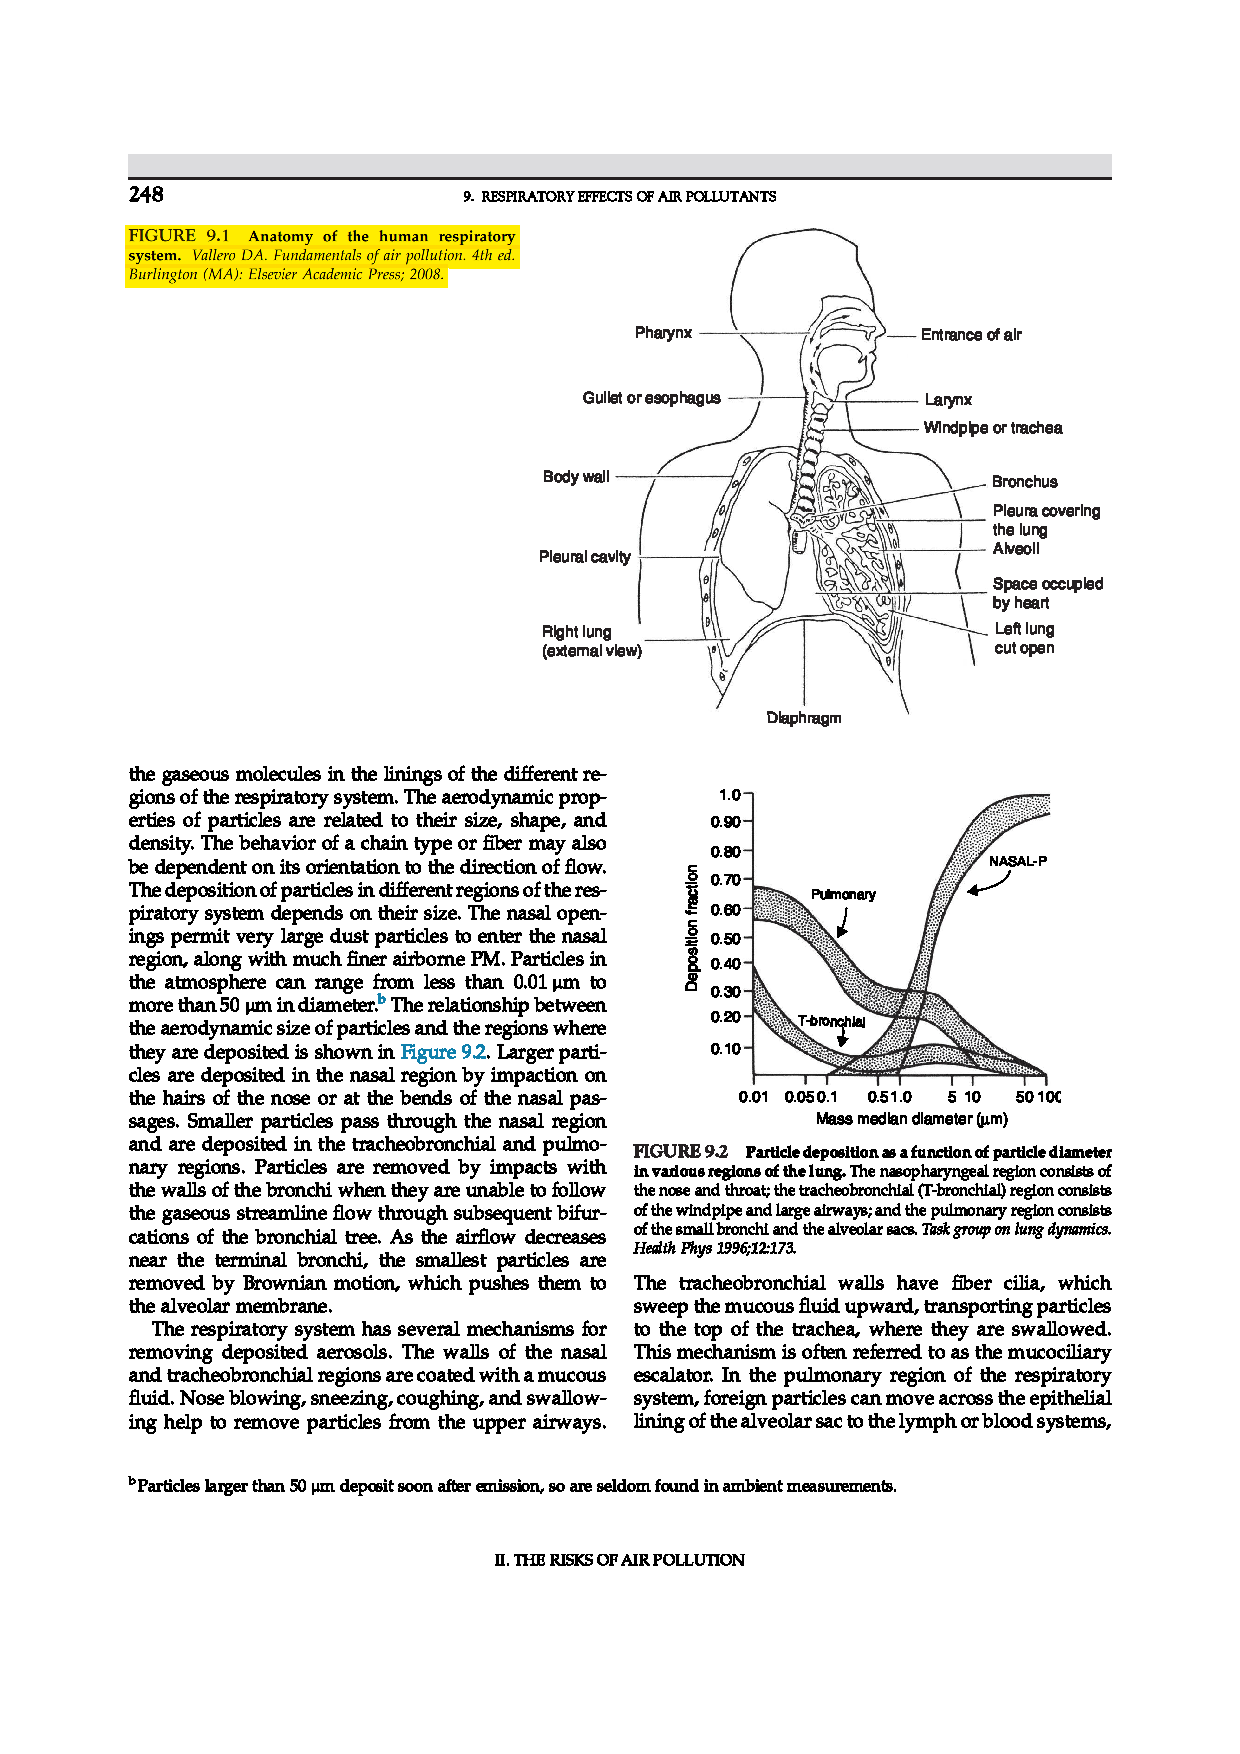
\includegraphics[clip,%
    trim=9.1cm 17cm 2.1cm 5cm,%
    width=.8\textwidth]{img/pdf/respiratory_system.pdf}
    \caption{Annotated anatomy of the respiratory
    system~\cite{Vallero2014}.}
    \label{fig:respiratory_system}
\end{figure}

The respiratory system has several (imperfect) mechanisms in place to
prevent particles from reaching the blood stream. Larger particles are
deposited in the nose, by impaction on the hairs and bends of the nose.
Smaller particles are immune to this first barrier, and manage to get to
the trachea and bronchi, where they are filtered also by impaction, this
time on the walls of the innumerable bifurcations of the bronchial tree.
The smallest particles are removed through Brownian motion, which ends
up pushing them against the alveolar membrane. Deposited substances are
then removed through the action of cilia in the pulmonary system's walls
or by coughing, sneezing or blowing one's nose~\cite{Vallero2014}.

While the body is quite efficient at filtering out particles from the
respiration process, the same cannot be said about gaseous pollutants.
Removal of these compounds can only be achieved through absorption,
which depends almost exclusively in the gases' solubility. High
solubility compounds are absorbed directly in the upper airways
(SO\textsubscript{2}, for instance), while less soluble gases (such as
O\textsubscript{3} and NO\textsubscript{2}) are absorbed in the lungs
themselves. Irritant gases trigger a variety of responses, in which one
can include sneezing, coughing or bronchoconstriction. These gaseous
compounds are then diffused through to the bloodstream or the lungs
themselves try to convert them into other substances via biochemical
processes. In some cases, this attempt to detoxify a pollutant can lead
to much more problematic circumstances. For instance, the lung is known
to active procarcinogenics, substances that are only carcinogenic after
being metabolized in a certain way~\cite{Vallero2014}.

Acute symptoms of \gls{AP} exposure are very varied, and range from mild
irritation to complete respiratory failure, depending mostly on level of
exposure and individual sensitivity to the chemical compound. One of the
most important acute manifestations of \gls{AP} exposure are encompassed
within the \gls{ALRI} group. There are several studies in which the
relationship between this issue and \gls{AP} is deducted and explained,
mostly in developing countries, and it remains as one of the major
causes for infantile death~\cite{CABI2019, UNICEF2013}. Children are one
of the most affected demographics by \gls{AP}~\cite{EEA2016}, and one of
the chief reasons for this is that the human respiratory system is till
developing in this stage of life.

In a 2016 review~\cite{Goldizen2016}, the authors searched the
literature for childhood adverse effects of \gls{AP}, with a particular
focus on respiratory problems. They have found evidence for a number of
respiratory complications and diseases that were previously reported in
the literature caused or exacerbated by \gls{AP}. Effects are many, and
vary immensely in nature, severity and affected populations. Short term
effects, like coughing and wheezing were found for the three types of
major pollutant and several others; several papers mention an
association between the occurrence of respiratory infections and
exposure to \gls{AP}, namely concerning \gls{PM} and \gls{no2}.  The
same review found reports of decreased lung function in children and
asthma exacerbation in children due to \acrlong{AP}. Moreover, a person
exposed to high levels of \gls{AP} during childhood are also more likely
to develop syndromes like \gls{COPD}, and to have exacerbated symptoms
of this disease. Finally, and perhaps more concerning, the carcinogenic
nature of several of the constituents of \gls{AP} leads to findings
relating the appearance of respiratory cancers to exposure levels during
childhood. Many of the conclusions of this review come from a
large-scale European effort called \gls{escape}, that intended to
investigate long-term health effects of \gls{AP} in Europe. \gls{escape}
was an \gls{fp7} initiative that ended in 2014.

\subsubsection{\acrlong{AP} and cardiovascular issues}%
\label{ssub:ap_and_cardiovascular_issues}

After being absorbed by the respiratory system, oxygen is distributed to
all cells of the body through the cardiovascular system. Air pollutants,
like particles and trace gases, are also capable of penetrating the lung
barrier and therefore share the same fate. There are several pathways
with which \gls{AP} and negatively affect the cardiovascular system. The
most immediate of which is probably an imbalance in the \gls{ans} caused
by direct inflammation and oxidative stress in the respiratory system.
The second most immediate pathway is systemic inflammation caused by
\acrlong{AP}. Finally, soluble \gls{AP} compounds in the bloodstream
also contribute to \gls{cvd} by increasing inflammation and oxidative
stress in the cardiovascular system~\cite{Brook2008, Vallero2014}.

The link between Air Pollution and cardiovascular effects started being
made during the twentieth century, given a series of incidents (like
London's 1952 killer-smog) that happened in the urban areas of
industrialized countries. Nowadays, \gls{cvm} has been shown to be
intricately connected to \gls{AP}. In fact, in a 2013 review indicated
that an annual increase of 10$\mu g / m^{3}$ in fine \gls{PM} and
NO\textsubscript{2} led to an increase of 11\% and 13\% respectively in
terms of \gls{cvm} and premature atherosclerosis, in spite of absolute
\gls{AP} concentrations were maintained below the European
policy-recommended thresholds. Road traffic exposure studies have
reported similar findings, with subjects having increased coronary
calcium scores~\cite{Bourdrel2017}.

Arrhythmia is one of the other cardiovascular issues that might be
caused by \gls{AP}. There is still some debate regarding whether or not
there is a causal relationship between the two, but there have been
several studies in which increased levels of \acrlong{AP} were
correlated with arrhythmia-related hospital admissions. Moreover, there
seems to be a correlation between low heart rate variability and
\gls{AP}, which is considered a marker for \gls{ans} imbalance and an
important risk factor for \gls{cvm}\cite{Bourdrel2017}.

The risk of stroke is also clearly exacerbated by the presence of
increased levels of \gls{AP}. In fact, it is currently thought that
\gls{AP} is responsible for about 29\% of the burden of stroke,
globally. Studies have shown that an increase of 5 $\mu g / m^{3}$ in
the annual \gls{PM}\textsubscript{2.5} concentration leads to a
remarkable 19\% increase in the risk of stroke, which was found to be
more significant in non-smokers. A positive correlation was also found
between gaseous pollutants (no\textsubscript{2}, CO and
SO\textsubscript{2}) concentration and the risk of stroke or stroke
mortality.

Short term effects of \gls{AP} on the cardiovascular system seem to be
predominantly the triggering acute coronary incidents. For instance, a
positive correlation was found between short term increases in \gls{AP}
and non-fatal myocardial infarctions.

\subsubsection{Gestational and developmental complications}%
\label{ssub:gestational_and_developmental_complications}

Mammals are in their life's most vulnerable stage while they are still
developing inside their mother's womb. This is the time when there is a
greater rate of tissue expansion and creation, creating an enormous need
for nutrients. These are supplied by the mother's blood, crossing the
placenta and reaching the fetus through its umbilical cord. High rates
of tissue formation and proliferation render the forming being unstable
and therefore more susceptible to the appearance of some kind of
morphological abnormality. At this time, there is no separation between
the mother's blood and the fetus, meaning that whatever chemical reaches
the progenitor's bloodstream also reaches the growing fetus. If the
mother is exposed, so is the fetus~\cite{Vallero2014}.

There are numerous chemicals that can affect the female reproductive
system, of which some are habitual components of \gls{AP}. They have
been associated to several highly adverse affects, and interfere with
such things as the processes by which the body is able to produce eggs,
or other processes that enable the formation of a single cell by the
union of the sperm and the egg (the zygote). After conception, \gls{AP}
has been known to reduce uterine nurturing capabilities, and hinder the
new being's development. Some of them are even teratogens, meaning that
they induce birth defects. Figure~\ref{fig:AP_in_utero} illustrates the
kind of defects that come with exposure, according to the time at which
the mother was exposed.

\begin{figure}[htpb]
    \centering
    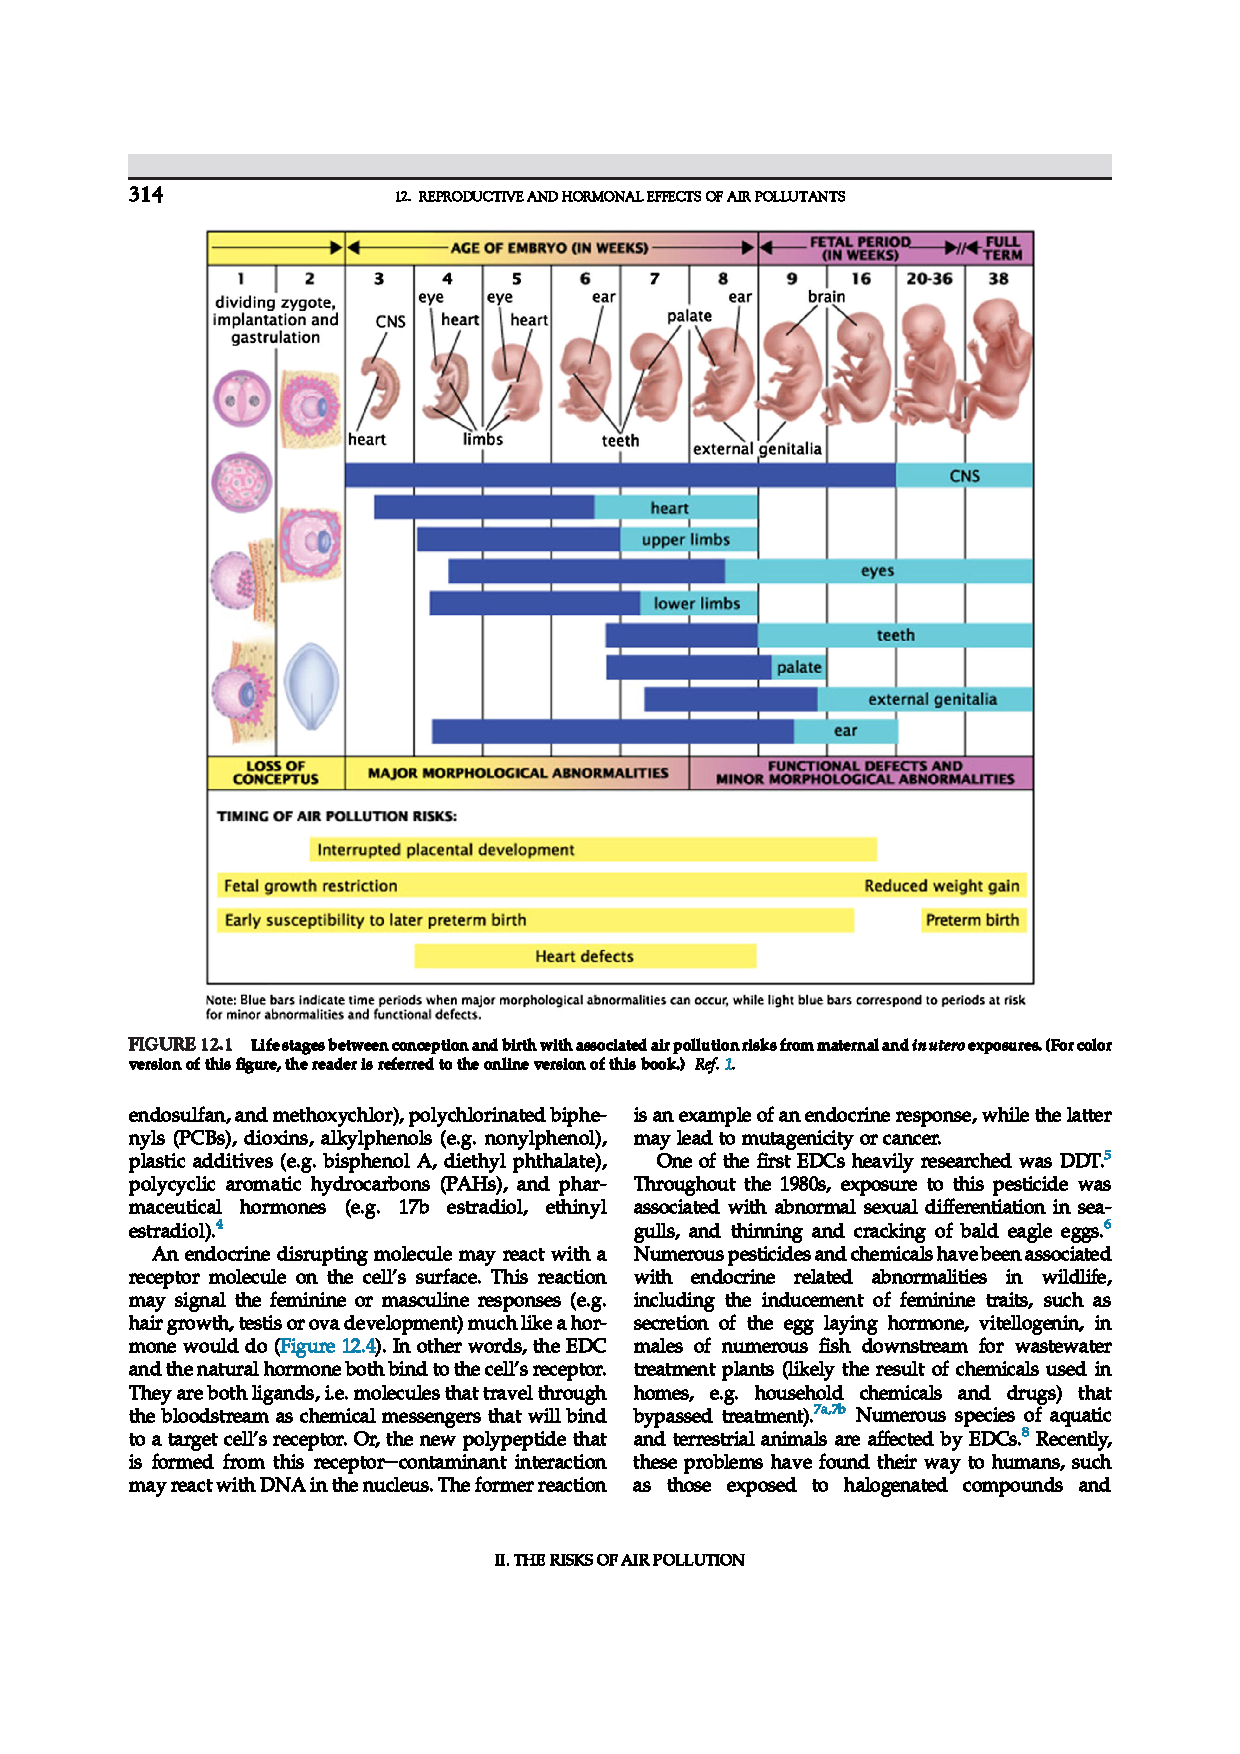
\includegraphics[clip,%
        trim=3.4cm 12.2cm 3.4cm 3.6cm,%
        width=0.8\textwidth]{img/pdf/development.pdf}
    \caption{Possible abnormalities caused by \gls{AP} exposure \emph{in
    utero}. Notice that time of exposure is of critical
    importance~\cite{Vallero2014}.}
    \label{fig:AP_in_utero}
\end{figure}

There are already several studies that correlate higher \gls{AP}
exposure levels to birth defects or the probability of negative
outcomes. For instance, in~\cite{Li2019}, researchers have studied the
association between \gls{AP} exposure levels (for the mother) and the
appearance of premature \gls{sga} by collecting more than 40000 births
in Changzhou Maternity (China) and studying the mother's typical
environment. This study has found a positive association between
\gls{sga} and exposure to \gls{PM}\textsubscript{2.5} in two or three
pollutants models of \gls{AP} (with \gls{no2} and \gls{so2}), during the
third trimester of gestation. Another, perhaps more comprehensive study,
was performed using Swedish data from 1997 to 2007, and found that there
was a positive association between \gls{o3} exposure and the appearance
of pre-eclampsia (a potentially deadly complication of pregnancy),
estimating that about 1 in 20 pre-eclampsia cases were caused by
\gls{AP}~\cite{Olsson2013}.

Besides uterine development compromises, birth defects and reproductive
difficulties, \acrlong{AP} has also been associated with hindrances to
the child's neurodevelopment. In a New York study was able to associate
lower levels of mental development at age 3, in African-American
children with valid prenatal \gls{pah} exposure data. In another study
from the neighboring Boston, \gls{AP} was associated with generally lower
cognitive test scores, even when correcting for several influencing
factors. On a different level, \gls{AP} was shown to produce significant
delays in the central conduction times of \gls{baep} tests in children,
indicating that there might be important repercussions of \gls{AP} to
vestibular and auditory development.

Although most other systems are affected by \gls{AP}, it does have a
particularly heavy toll on the respiratory development. This is because
the lungs are not completely developed at birth, and are only finished
in the late teens. The level to which \gls{AP} affects the respiratory
system development varies greatly with the staeg of life in which the
effect is produced, and severity is also very varied. Acute negative
effects range from respiratory death to chronic
cough~\cite{Vallero2014}. Moreover, childhood (and prenatal) exposure to
\gls{AP} has been associated with the emergence of conditions such as
\gls{COPD} and asthma.

\begin{figure}[htpb]
    \centering
    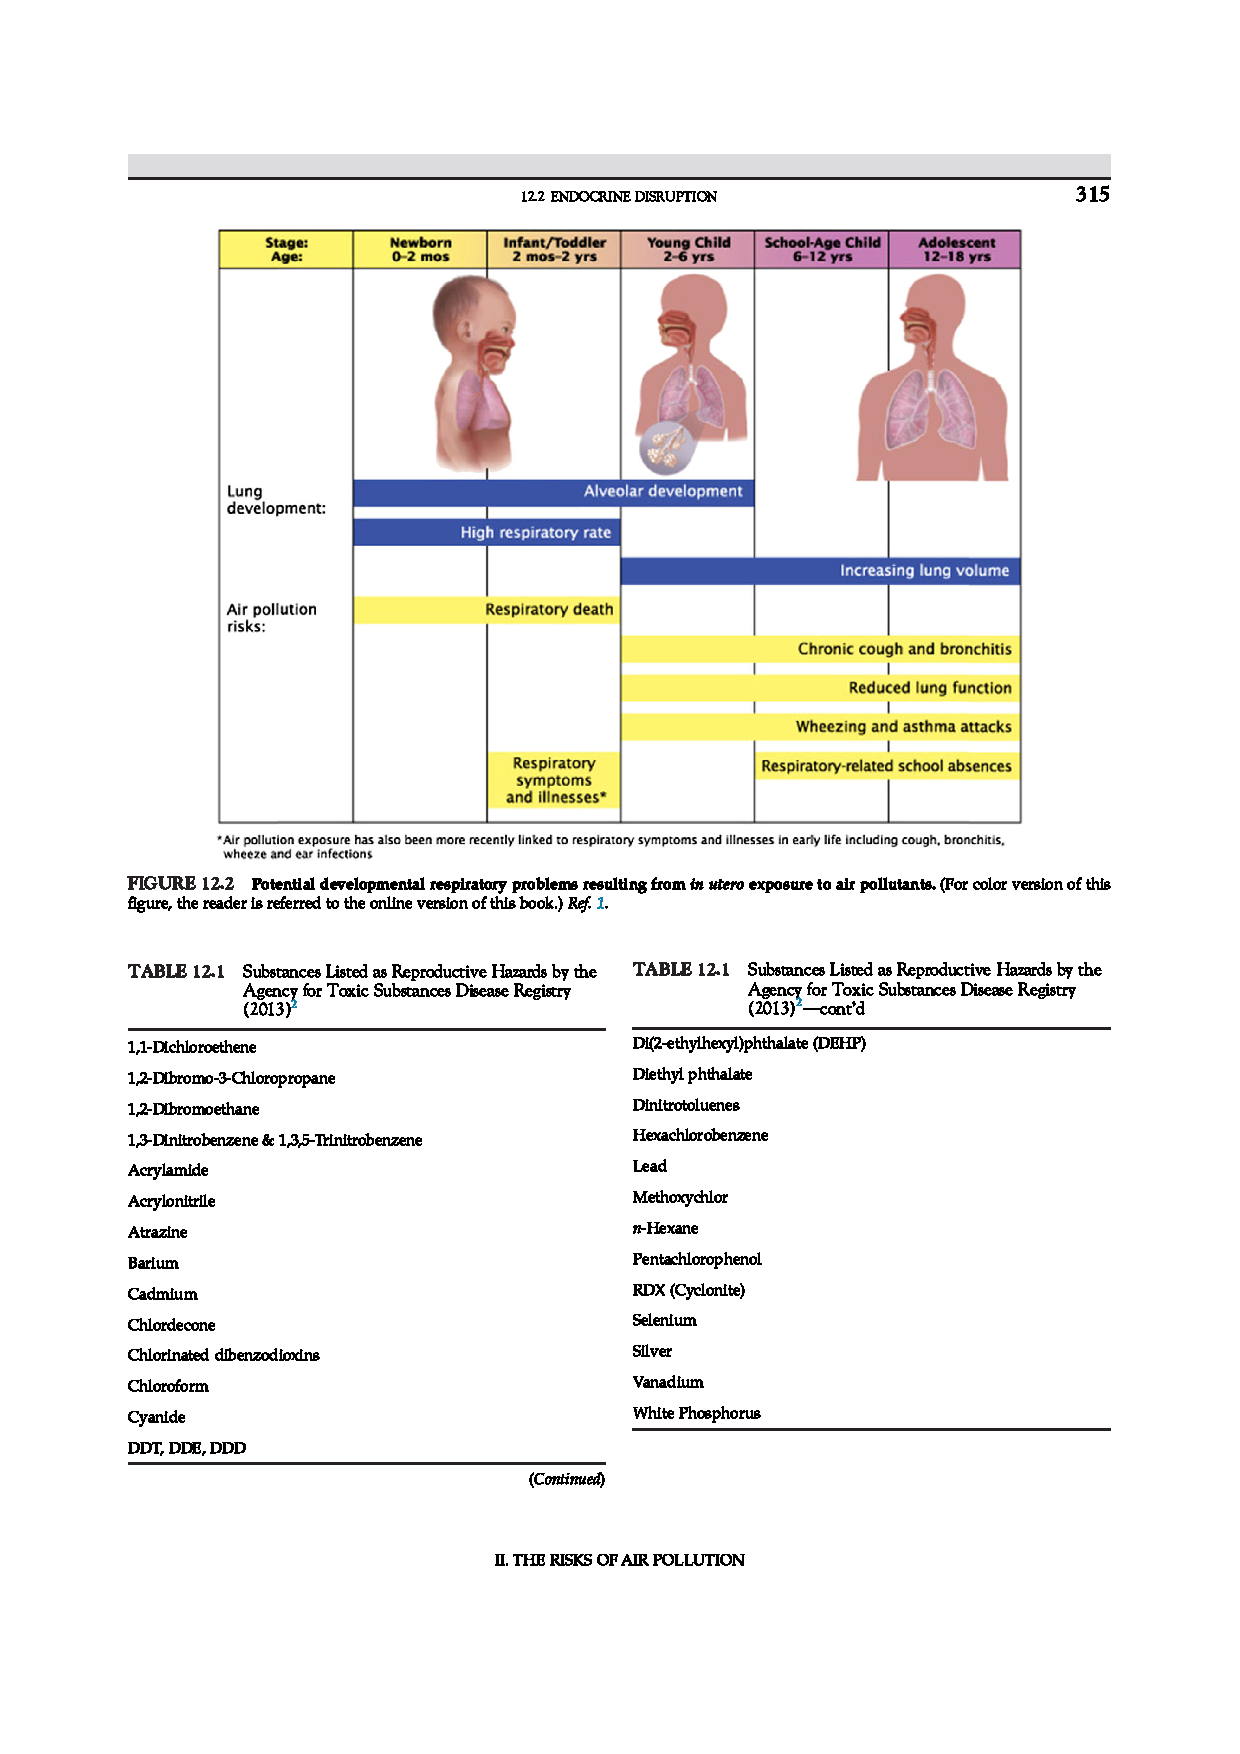
\includegraphics[clip,%
        trim=3.4cm 15cm 3.4cm 3.6cm,%
        width=0.8\textwidth]{img/pdf/lung_development.pdf}
    \caption{Developmental stages of the lung throughout life vs the
    risks of \gls{AP} exposure in each stage~\cite{Vallero2014}.}
    \label{fig:img/lung_development}
\end{figure}

\subsubsection{Neurological disorders}%
\label{ssub:neurological_disorders}

The brain and the \gls{cns} were one of the last to be included in the
range of organs that are affected by \gls{AP}. While the effects of
\gls{AP} on the respiratory and cardiovascular systems are quite broad
and include some "surprises", the fact that these systems were affected
by \acrlong{AP} was evident and expectable, given the type of exposure
these systems endure. The \gls{cns}, on the other hand, has a more
difficult to express relationship with \gls{AP}, and has required more
sophisticated methods to detect~\cite{Vallero2014, Genc2012}. It was in
the beginning of this century that the first connections between
\gls{AP} and the emergence of neurological disorders started to be made,
and from then on, we have progressed into thinking that not only are
they related, but also that \gls{AP} might be one of the key driving
forces in the onset of certain neurological diseases, including the most
dreaded of them all, Alzheimer's and Parkinson's~\cite{Genc2012,
DePradoBert2018, Calderon-Garciduenas2014}.

The reason why \gls{AP} is able to reach and damage the \gls{cns} is a
continuation (or even an extension) of the ways in which it affects the
cardiovascular system. By crossing the alveolar barrier into the
bloodstream, \gls{AP} acts as an oxidative stress source. As it can also
do in lung tissue, \acrlong{AP} creates some local proinflammatory
effects in the cardiovascular system, affecting the vascular endothelium
cells. This can lead to a systemic inflammatory status, which is
accompanied by the production of proinflammatory cytokines (a type of
message-protein that is used by organisms to trigger certain types of
response, like inflammation~\cite{Zhang2007}). Now, since blood vessels in the
brain are extremely responsive to this kind of message, their presence
can activate cerebral endothelial cells and disrupt the blood-brain
barrier~\cite{Genc2012}.

In 2018, a consortium of several Spanish universities and researchers
wrote a review detailing the until-then-published articles dealing with
the neurological implications of \gls{AP}~\cite{DePradoBert2018}. This
review identifies several articles that connect the long-term exposure
to \acrlong{AP} with adverse impacts on the brain and brain structures.
\emph{In vitro} and \emph{in vivo} studies,  focusing on traffic related
emissions and their effect on gray matter cells, have found that these
display significant alterations. On other studies identified by the
review, it was shown that white matter, the myelinated part of the
brain, is particularly sensitive to \gls{AP} and its volume is
significantly decreased both in the elderly and children, as consequence
of prolonged exposure to it. 

There are also several articles that show that there is an association
between exposure to air pollutants and impairments on brain function.
In Section~\ref{ssub:gestational_and_developmental_complications},  I
have already mentioned a study that was conducted in New York, and that
found that the children that they were using as subjects were found to
have measurable cognitive deficits in comparison with children of the
same age living in less polluted areas which are compatible with the
affected areas of the brain that were detected through neuroimaging
studies~\cite{DePradoBert2018}.

\subsection{\acrlong{AP} effects on ecosystems}%
\label{sub:ap_effects_on_ecosystems}
\todo[inline]{citations - vallero and lovett + european report}
The Earth is home to an almost unbelievable number of different
ecosystems. The ubiquitousness of \gls{AP} means that all of them are in
some way or another affected by this problem. In general terms, the
threat posed by \gls{AP} to any given habitat is a function of its
biodiversity, defined as the number of different living beings that
inhabit a certain environment (in all biological
kingdoms)~\cite{OxfordPress2020}. Living beings within an ecosystem are
like nodes in a graph, with many connections to any particular node.
More biodiversity corresponds to a greater number of nodes and an even
larger number of links,  which means that there is a greater probability
that some of those links become disrupted by \acrlong{AP} in some way.

Water based environments are greatly affected by \gls{AP}. Material
deposition on the surface of the water can have serious consequences in
terms of habitat conditions for holding life. In this regard, the most
important air pollutants are \gls{no2} and \gls{so2},  which
significantly decreases the water's pH. On its own, this represents a
major problem. The acidifying effects of nitrogen and sulfur deposition
became very pronounced in Scandinavia (among other places). Thousands of
this territory's lakes, once teeming with wildlife, became effectively
lifeless. Those that did not reach this point, have seen the number of
fish living on their waters dwindle to numbers from which there may be
no return~\cite{DeWit2015}. Sulfur and nitrogen depositions also enrich
surface waters, altering the solubility and other physical aspects on
the surface of the water, which in turn inevitably leads to disruptions
in species abundance and diversity. Moreover, indirect effects may also
take their tolls. For instance, \gls{o3} does not play any significant
role in the chemical behavior of a water body, but it can influence the
number of predators around this habitat, which will compromise the
predator-prey balance of the aquatic environment~\cite{Vallero2014,
Lovett2009}.

In terrestrial ecosystems, \gls{AP} effects are not smaller in
importance or complexity, and they are different for each type of being.
To the Flora, \gls{AP} can have a subtle to deadly effect, depending on
variables like pollutant chemical species, exposure time, or plant life
stage in which exposure happens. For instance, \gls{o3} is especially
poisonous to plants. Even small concentrations of this gas will cause
plant growth to decrease significantly. It enters the plant through the
stomata and reduces photosynthesis through increased oxidative stress.
Many times, although concentrations are not enough to outright kill the
plant, they are enough to make them more susceptible to other attacks
like pathogens, insects or environmental conditions. \acrlong{o3} is
commonly responsible for huge financial losses that come from the
diminished agricultural yields. And while it is true that due to several
policies, \gls{AP} is in a clear downward trend since the 1980s in urban
regions, it is also true that in many rural areas, these changes have
been smaller or non-existent, making these losses even more relevant.

Forests are among the most susceptible environments to \gls{AP}. They
suffer from the previously described mechanisms of \gls{AP} damage, like
acidic deposition, but also suffer from other, less direct pollution
risks. Emission of greenhouse gases can induce changes in humidity,
temperature, and general climate profile of a forest. The combination of
direct and indirect risks result in an exacerbation of both, leading to
more and more forest losses due to \acrlong{AP}. The damage done to
forests all around the world is especially problematic given the
biodiversity that these ecosystems contain within themselves.
Rainforests in particular are thought to contain more than half of the
world's terrestrial species. These species have many times adapted to a
particular kind of microhabitat which only exists in the specific
rainforest in which it lives. Changes in these specific conditions,
whether caused by \acrlong{AP} or any other cause, are leading to
alarming extinction rates in forests and rainforests globally.

Of course it is not only the flora that suffers with \acrlong{AP}.
Direct implications of \gls{AP} on animals approximate those that fall
upon humans. We are an animal species, after all. Our main difference is
the adaptation capabilities that our superior intellect grants us, which
allows us to escape more or less unscathed for a longer period of time,
and to combat what we cannot escape from in ways which are simply
unaccessible to other animal species. So, although \gls{AP} has direct
effects on all animals that are exposed to it, ecosystem damage and
eventual destruction remains the most perilous factor for this
biological realm~\todo{should I get another source on this problem? }.





\subsection{\acrlong{AP} Sources}%
\label{sub:ap_sources}

There are almost as many \gls{AP} sources as there are pollutants. The
first major division between these sources is whether they are natural
or anthropogenic. However, this separation is not always clear, as one
source can lead to another and boundaries become fuzzy within their own
context. The most prominent example of such is the case of accidental
fires. While they are most of the times classified as a natural source
of \gls{AP}, their origin lies most of the times in human activities. In
this section, I will present a selection of the most important naturally
occurring air pollutants and examples of how they have affected human
lives throughout the times. The selection itself does not intend to be
complete description of pollution sources, but rather paint a general
picture of the subject.

\subsubsection{Natural Sources of \acrlong{AP}}%
\label{ssub:natural_sources_of_ap}

Although people, governments and institutions tend to speak far more
seldomly of them than of their man-made counterparts, natural sources of
air pollutant are not only abundant, but also important. One of the main
natural sources of \gls{AP} are volcanic eruptions. These phenomena are
responsible for the emission of immense quantities of \gls{PM} and gases
such as \gls{so2}, \gls{h2s} and methane. Depending on the type of
volcanic eruption, the emitted cloud of gas and \gls{PM} can remain
airborne for long periods of time, even disrupting modern life at times,
namely in what concerns air travel. The last eruption to happen in
Portuguese soil took place in the remote Azorian island of Faial. In
September 1957, the Earth shook almost continuously for around two
weeks. Finally, on the 27\textsuperscript{th}, 100 m Northeast the
Capelinhos islands, the sea was seen to boil and project vapor and
volcanic material hundreds of meters into the air. In the following
hours, the underwater volcano finally exploded, emitting large
quantities of volcanic ash and gases into the atmosphere. The phenomenon
lasted for more than a year, and the final ejection of lava took place
in October 1958 (see Figure~\ref{fig:capelinhos1957}). The eruption had
a significant social impact, in addition to its ecologic importance. In
the end, 40\% of Faial's population left the island as a
result~\cite{Vallero2014, TSF2017}.

\begin{figure}[htpb]
    \centering
    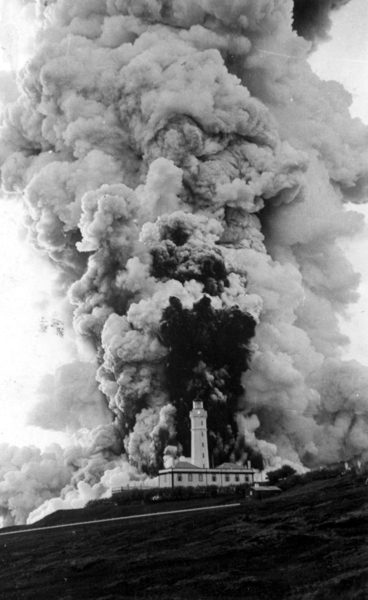
\includegraphics[width=0.8\linewidth]{img/jpg/capelinhos1957.jpeg}
    \caption{Dramatic photograph depicting the Capelinhos' lighthouse,
    half a kilometer from the eruption site, surrounded by a cloud of
    ash \gls{PM}, volcanic gas and water vapor with more than 1km in
    height\cite{TSF2017}.}
    \label{fig:capelinhos1957}
\end{figure}

Oceans are also a significant source of \gls{AP}. Aerosol particles of
salt are continuously emitted from these large masses of salt water,
which damage many human created structures, namely metallic
constructions. In certain parts of the world, another important source
of \acrlong{PM} (especially because of its consequences in the
inhabitants' daily life) are dust storms. The most famous of these
events, and one of the most deadly storms in the recorded history of the
US territory was the infamous \emph{Black Sunday} dust storm. Starting
on Palm Sunday, 14 April, this sky-blackening dust storm punished the
peoples from the panhandles of Texas and Oklahoma, burying entire houses
(see Figure~\ref{fig:dust1935}) under the dust and destroying the
livelihoods of thousands of Americans. Dust storms were an important
part of the US history during the 1930s and led to the creation of the
Soil Conservation Service, a branch of the US Department of
Agriculture~\cite{Vallero2014,Agriculture2012, Reis2008}.


\begin{figure}[htpb]
    \centering
    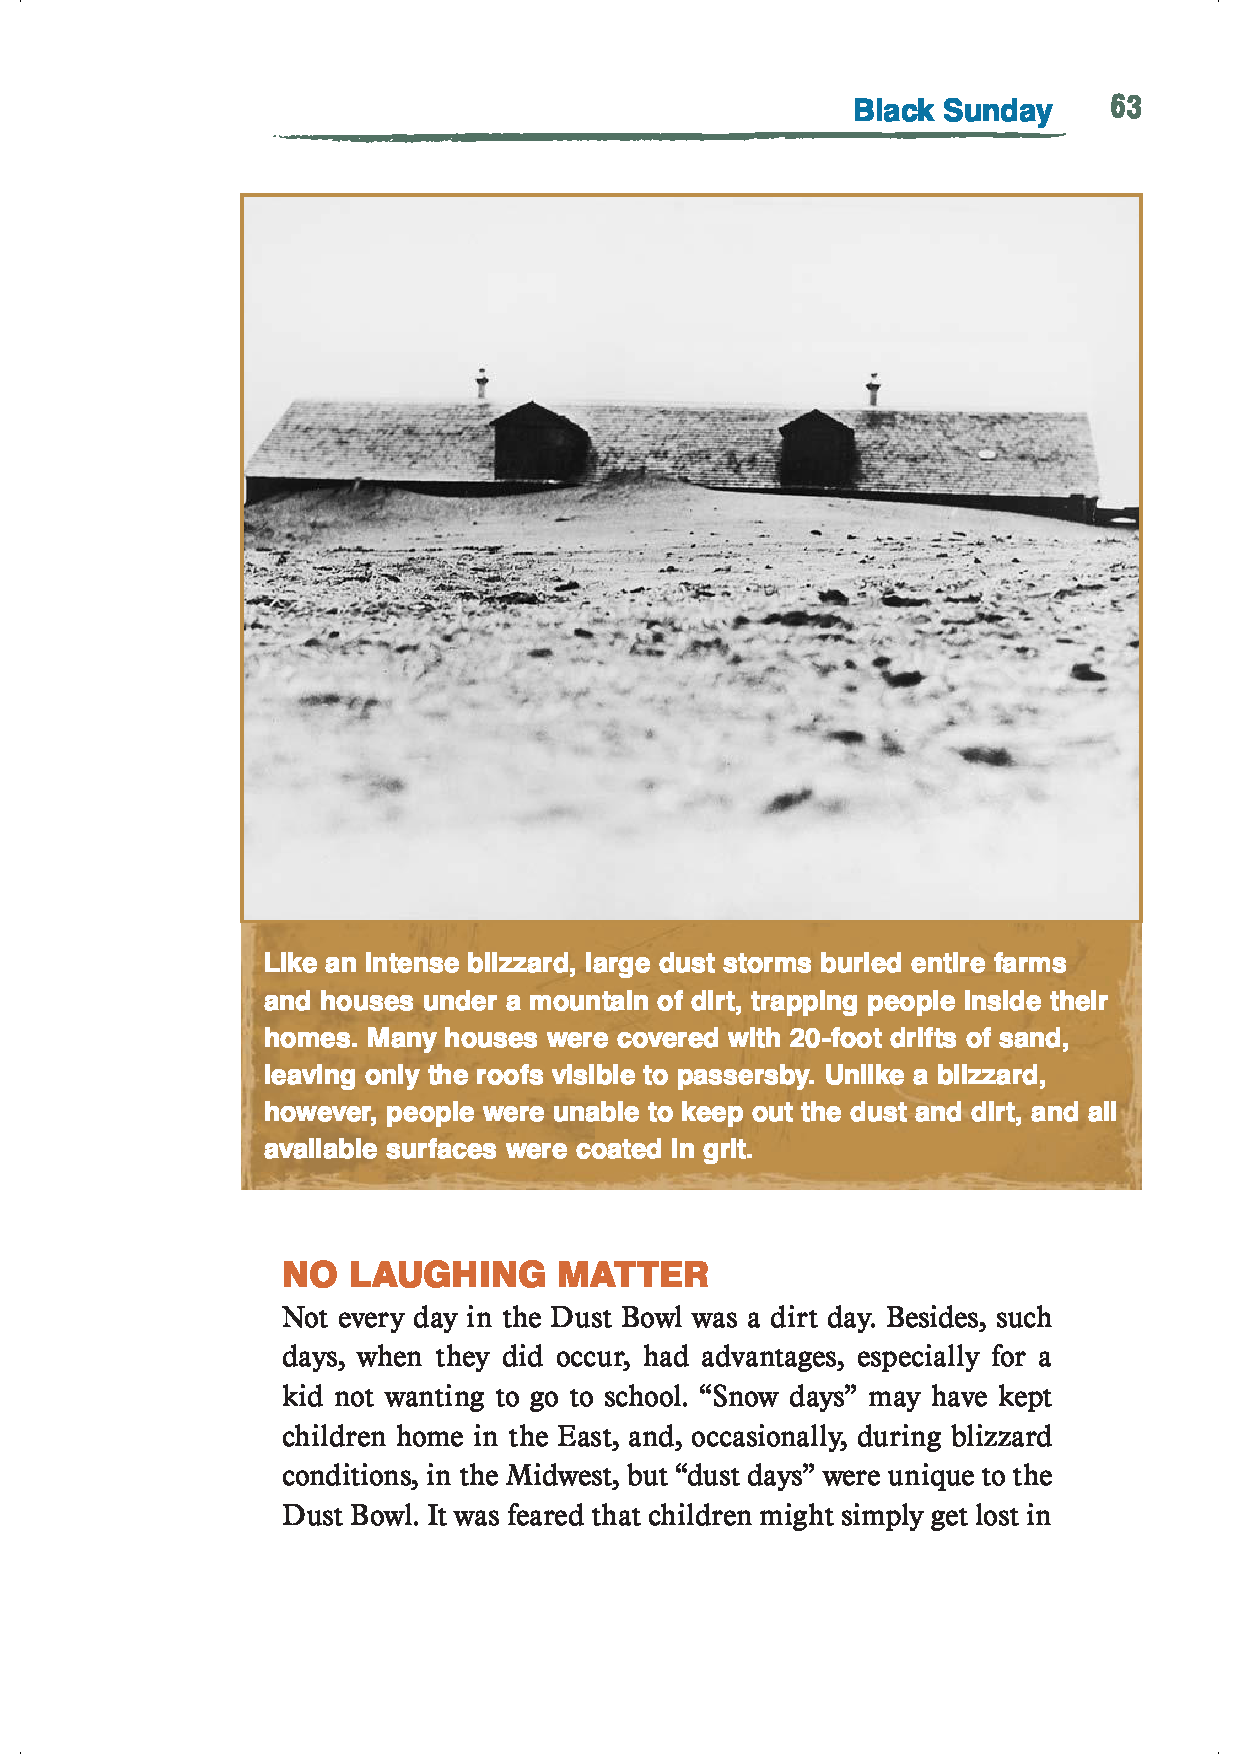
\includegraphics[clip,%
        trim=4.3cm 15cm 2cm 3.6cm,%
        width=0.8\textwidth]{img/pdf/dust.pdf}
        \caption{House almost completely buried by the Black Sunday dust
            storm. Several houses were entirely swallowed during this
            storm, trapping people inside, as if a big blizzard had hit
            them. Unlike a blizzard though, there was nothing anyone
            could do to keep the dirt outside, and all surfaces were
            covered black~\cite{Reis2008}.}
    \label{fig:dust1935}
\end{figure}

Fires are also one of the largest sources of natural air pollution in
the world. The uncontrolled burning of organic matter that is a large
forest fire creates a large quantity of air pollutants that range from
smoke to unburned (or partially burned) hydrocarbons, nitrogen and carbon
oxides, and ash particles. Besides the obvious dangers of this kind of
burnings for human life and activities, forest fires can also cause
indirect damages, such as disruptions in supplies and travel due to
reduced visibility~\cite{Vallero2014}.

Trees and forests in themselves are also responsible for a certain
quantity of air pollution. Although they have the main part in the
carbon dioxide conversion into oxygen, through photosynthesis, plants
and trees are still the largest emitters of hydrocarbons in the planet,
as attested by the blue haze that is visible on top heavily forested
areas, resulting from chemical reactions between \gls{VOC}s produced by
the trees. This counter-intuitive fact was in the origin of the infamous
Ronald Reagan speech in which he "blamed" trees for much of \gls{AP}, in
a time when anthropogenic \gls{AP} was at its apogee in the US and
Europe.Plants are also the emitters of another kind of \gls{PM}, which
is of particular importance both to themselves and humans, which are the
pollens. This is a bio-aerosol - a type of aerosol that is or was part
of a living being - associated with a number of
diseases~\cite{Vallero2014}.

Finally, I will discuss Radon gas. This is a natural occurring
radioactive gas that is part of the radiative decay of Uranium present
in all rocks. Although chemically inert, Radon is radioactive and, as
all radioactive substances, emits particles when it decays. Although
present virtually everywhere, outdoor concentrations of Radon are
typically too small to cause any problems. The problem with this gas
comes essentially from indoor concentrations, namely at home. Being a
gas, Radon is able to enter people's houses, exposing the inhabitants.
Prolonged exposure to Radon gas is the second biggest cause of lung
cancer and authorities estimate that between 3 and 14\% of lung cancer
cases are caused by this gas. In Portugal, Radon concentrations were
found to be below the European prescribed limit in two thirds of the
houses in a 2001 study, but in 17\% of the cases, concentrations were
not only above this limit, but also over the highest tolerable
limit~\cite{Vallero2014, WorldHealthOrganization2016, ProTeste2003}.


\subsubsection{Anthropogenic Sources of \acrlong{AP}}%
\label{ssub:anthropogenic_sources_of_ap}

\acrlong{AP} that originates from human activities is called
anthropogenic. Since the first industrial revolution, mankind has been
using more and more resources to fuel our progress and continuously
improving way of life. Of course, the consumption of natural resources
has some unpleasant and sometimes dangerous consequences. The most
important of which, looking from the lens of this thesis, is the
incredible increase in the levels of \gls{AP}. If one had any doubts
whatsoever, all it would take would be a look into the atmospheric
\gls{co2} concentration chart (Figure~\ref{fig:co2_concentration}) from
a few centuries back to the current day to completely dissipate them.

\begin{figure}[htpb]
    \centering
    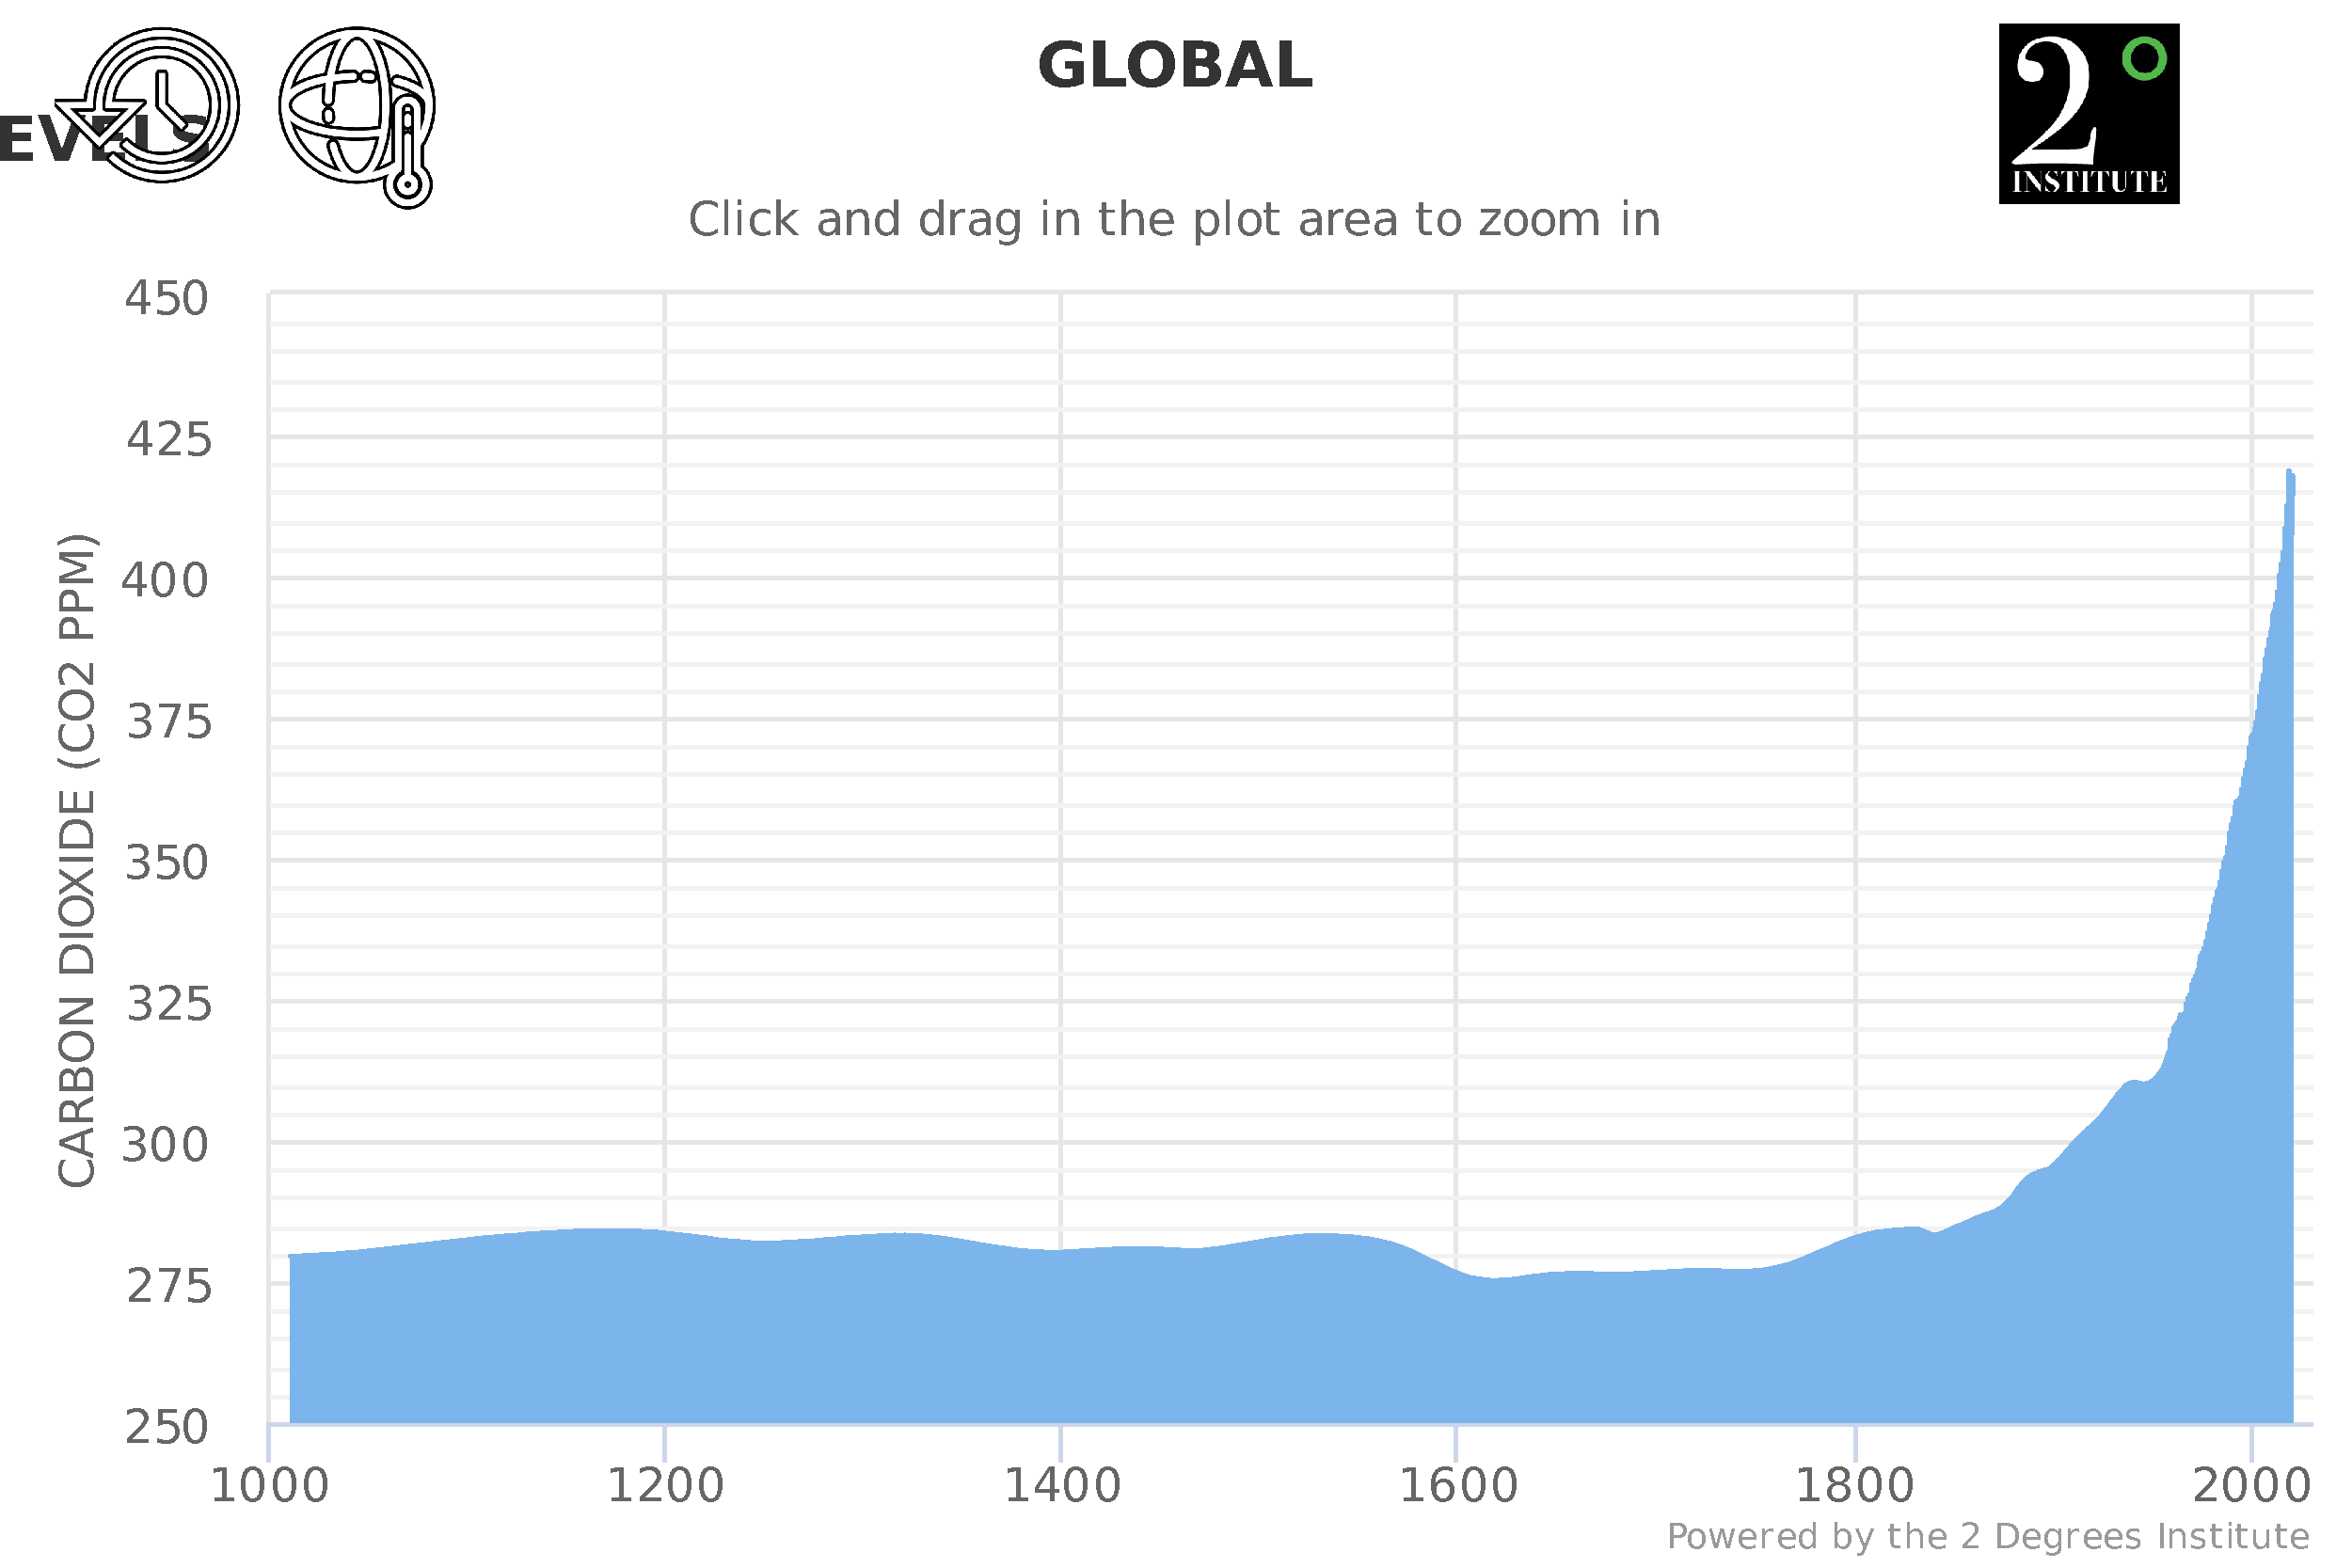
\includegraphics[clip, % left, bottom, right, top
                     trim=0cm 1cm 0cm 4.5cm,%
                     width=0.8\linewidth]{img/pdf/co2_ice_cores.pdf}
                     \caption{\gls{co2} atmospheric concentrations since
                         the year 1000. Note the seemingly exponential
                         increase since the 1800s. Plotted and published
                         by the 2 Degrees Institute~\cite{co2levels2020}
                         with data from ice cores~\cite{Etheridge} and
                         in situ monitors~\cite{Tans}.}
    \label{fig:co2_concentration}
\end{figure}

There are literally hundreds of sources of \gls{AP}, but it is possible
to categorize them into 4 main \emph{families}: industrial processes,
energy (includes transportation), agriculture and forestry, and waste.
Of these 4 broad categories, as displayed in
Figure~\ref{fig:anthropogenic_pollution_categories}. The most prominent
is without a doubt the energy sector, although we also have to bear in
mind that any and all combustion used in the other sectors is counted as
energy production~\cite{InternationalAgencyforResearchonCancer2016,
CABI2019}.\todo{table with major pollutants?}

\begin{figure}[htpb]
    \centering
    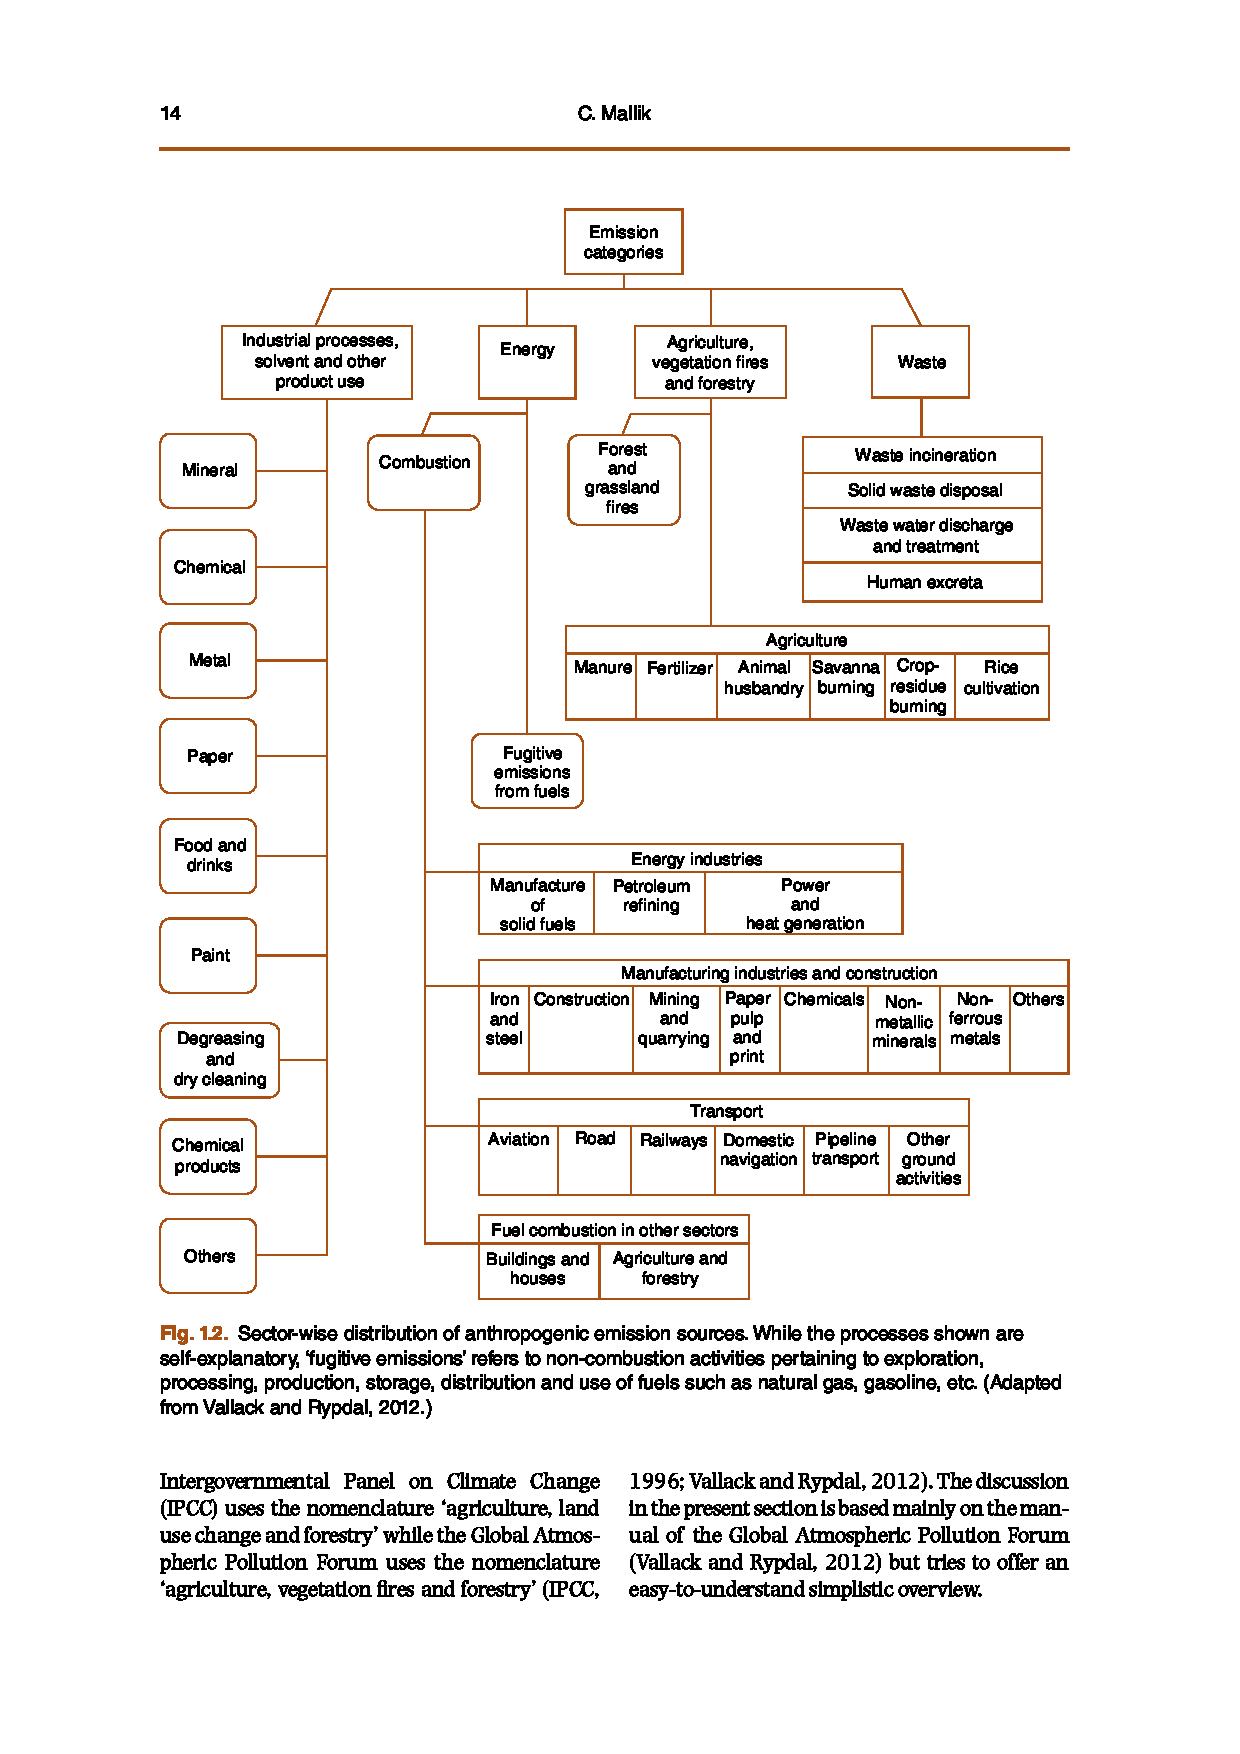
\includegraphics[clip,% left, bottom, right, top
        trim=2.3cm 7.3cm 2.3cm 2.6cm,%
        width=\textwidth]{img/pdf/pollution_sources.pdf}
    \caption{Schematic presentation on the sources of anthropogenic
    pollution and its categorisation according to the IPCC. Adapted
    from~\cite{CABI2019}}
    \label{fig:anthropogenic_pollution_categories}
\end{figure}

From 2002 to 2011, fossil fuel combustion has been responsible for an
average of 8.3 petagrams of carbon per year. This truly gigantic carbon
footprint is in its majority explained by the worlds energy needs, which
are ever increasing up to now. In 1990, total energy demand was situated
at 356 quadrillion \gls{btu}, having grown to 410 quadrillion \gls{btu}
in 2010. In 2020, energy demand estimates are located at 600 quadrillion
\gls{btu}, of which almost a quarter was expended by
China~\cite{CABI2019}.

It is important that we focus a little bit more on the Chinese case. It
is now somewhat near commonsense to regard China as the factory of the
world, and this of course is tied to Chinese energy consumption and
production. On the same line of reasoning, this must mean that in some
way, the country's energy expenditure is connected to the amount of
financial resources that it produces, the \gls{gdp}. Looking at the
plots in Figure~\ref{fig:china_energy}, one can see that all these
numbers are highly correlated. When we ponder on the case of Chinese
\gls{AP}, and wonder why has this problem not been addressed previously,
given its imposing dimensions and growing importance, one must take into
account that, given the indirect importance of \gls{AP} on Chinese
people's gains, it is highly likely that the country's governments will
be reluctant to decrease it in any expedient form~\cite{CABI2019, IEA,
WorldBank}.

\begin{figure}[htpb]
    \centering
    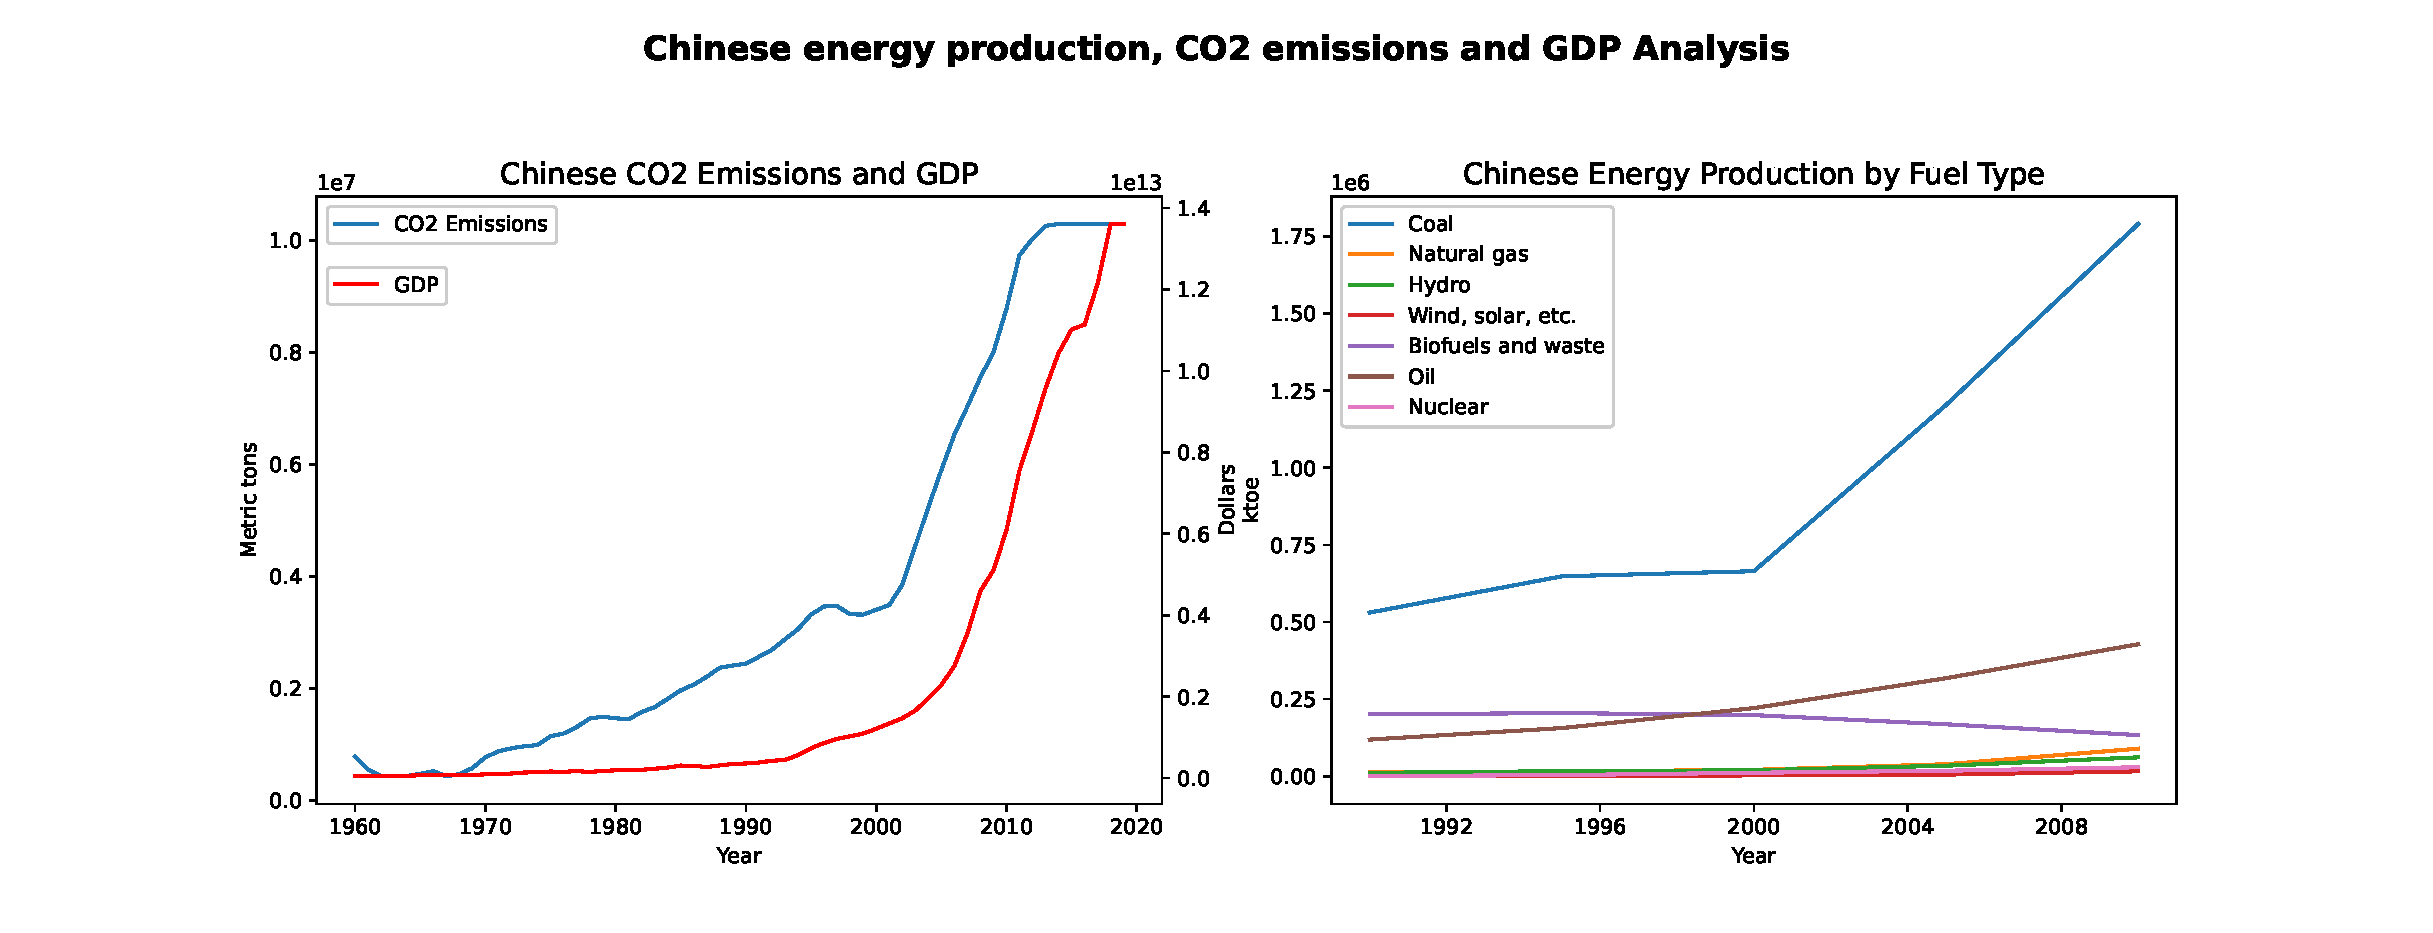
\includegraphics[width=\linewidth]{img/eps/energy_co2_gdp.eps}
    \caption{Chinese energy production, \gls{gdp} and \gls{co2}
    emissions.  Data collected from the World Bank and International
    Energy Agency websites~\cite{WorldBank, IEA}}
    \label{fig:china_energy}
\end{figure}

Another important conclusion that we can take from the plot in
Figure~\ref{fig:china_energy} is that China has a large and historical
dependence on the use of coal as fuel for energy production. This adds
to the problem described in the above paragraphs, as coal is the single
most damaging fossil fuel available. Not only does China get most of its
energy from coal burning, but is also responsible for more than half of
the worlds production and consumption of this substance (see
Table~\ref{tab:global_energy_consumption}).


\begin{table}[htpb]
    \centering
    \small
    \caption{Global energy production, divided according to the fuel
    used to obtain it and the production country.}
    \label{tab:global_energy_consumption}
    \begin{tabularx}{\textwidth}{lXXXXX}
    \toprule
    \textbf{Country} & \textbf{Liq. Fuel} &
    \textbf{Coal} & \textbf{Nat. Gas} &
    \textbf{Renew.} & \textbf{Nuc.} \\ 
                    &\textbf{\tiny{(M barrels /
    day)}}&\textbf{\tiny{(BTU)}}&\textbf{\tiny{(T cu.
                    ft)}}&\textbf{\tiny{(BTU)}}&\textbf{\tiny{(b kWh)}}\\\midrule
    \textbf{China} & 10,6 & 80,6 & 5,1 & 10,6 & 93 \\
    \textbf{USA} & 18,5 & 17,3 & 25,5 & 7,8 & 769 \\
    \textbf{Europe} & 14,4 & 12,5 & 17,9 & 11,7 & 837 \\
    \textbf{Middle East} & 16 & 0,1 & 14,8 & 0,2 & 1 \\
    \textbf{India} & 3,6 & 12,6 & 2,1 & 3,5 & 30 \\
    \textbf{Russia} & 3,4 & 4,5 & 15,7 & 1,7 & 166 \\
    \textbf{Africa} & 3,5 & 4,3 & 2,7 & 4,7 & 12 \\
    \textbf{Brazil} & 3,3 & 0,5 & 1,1 & 6,8 & 15 \\
    \textbf{World} & 91,4 & 153,9 & 120,8 & 63,7 & 2345 \\ \bottomrule
    \end{tabularx}
\end{table}

\gls{ice} are the single most important means for powering human
transportation. Almost every vehicle in the world uses a kind of
\gls{ice}. These motors operation is an application of the Otto cycle,
in which the chemical energy in the fuel is converted to mechanical
energy. These engines are as ubiquitous as the fossil fuels that have
powered them since the beginning of the automobile revolution, in the
early 20\textsuperscript{th} century. Fossil fuels have several features
that make them ideal to power our vehicles. Their energy density is
generally high~\todo{citation and examples}, they are incredibly safe to
manipulate and use, and fossil fuel infrastructure can be found in
almost every far corner of the Earth. However, using them releases a
number of gaseous and particle-condensed side products into the
atmosphere, and this makes traffic one of the most important sources of
\gls{AP}. For instance, traffic pollution is the main responsible for
human exposure to \gls{nox} gases. Without countermeasures, gasoline
\gls{ice} equipping passenger vehicles emit around 1.8 g/km of these
gases, while diesel emits 2.8 g/km and \gls{gpl} around 2.1 g/km. On
heavy duty engines, like on trucks and tractors, these figures skyrocket
to 14.7 g/km for diesel engines and around 5.1 g/km for
\gls{gpl}~\cite{CABI2019}.

Energy production (including transportation) is clearly the single
largest contributor to global \gls{AP}. This does not mean that other
human activities do not pollute or produce air pollutants. Pollutant
contributions from the industry, the agricultural activities and waste
disposal are also non-negligible. In fact, industries around the world
are responsible for the production and emission of all the criteria
pollutants. It is important to single out one particular activity, which
is the burning of forest for land-use changes. \gls{co} emissions for
this purpose are very high due to the nature of the burning material,
which emits more than 50 times more \gls{co} than fuel or
coal~\cite{CABI2019}.

\subsubsection{The European Case}%
\label{ssub:the_european_case}

Europe has for long been on the forefront of the fight against \gls{AP}
emissions. The European Union has put in place a number of policies
aiming at cutting (or even eliminating) emissions of human health
compromising pollutant components. Few places in the world have been so
demanding regarding their environmental practices, and numbers are a
clear reflection of these adaptation efforts. In their 2019 report, the
\gls{EEA} state that European emissions have globally declined, and have
been declining since at least the year 2000. Moreover, and in contrast
with China's case, the \gls{gdp} does no seem to be connected to
\gls{AP} emissions. As can be seen in
Figure~\ref{fig:european_emission_trends}, emissions are decoupled from
economic growth, as there are now less emissions per \gls{gdp} unit than
before~\cite{EEA2019}.

\begin{figure}[htpb]
    \centering
    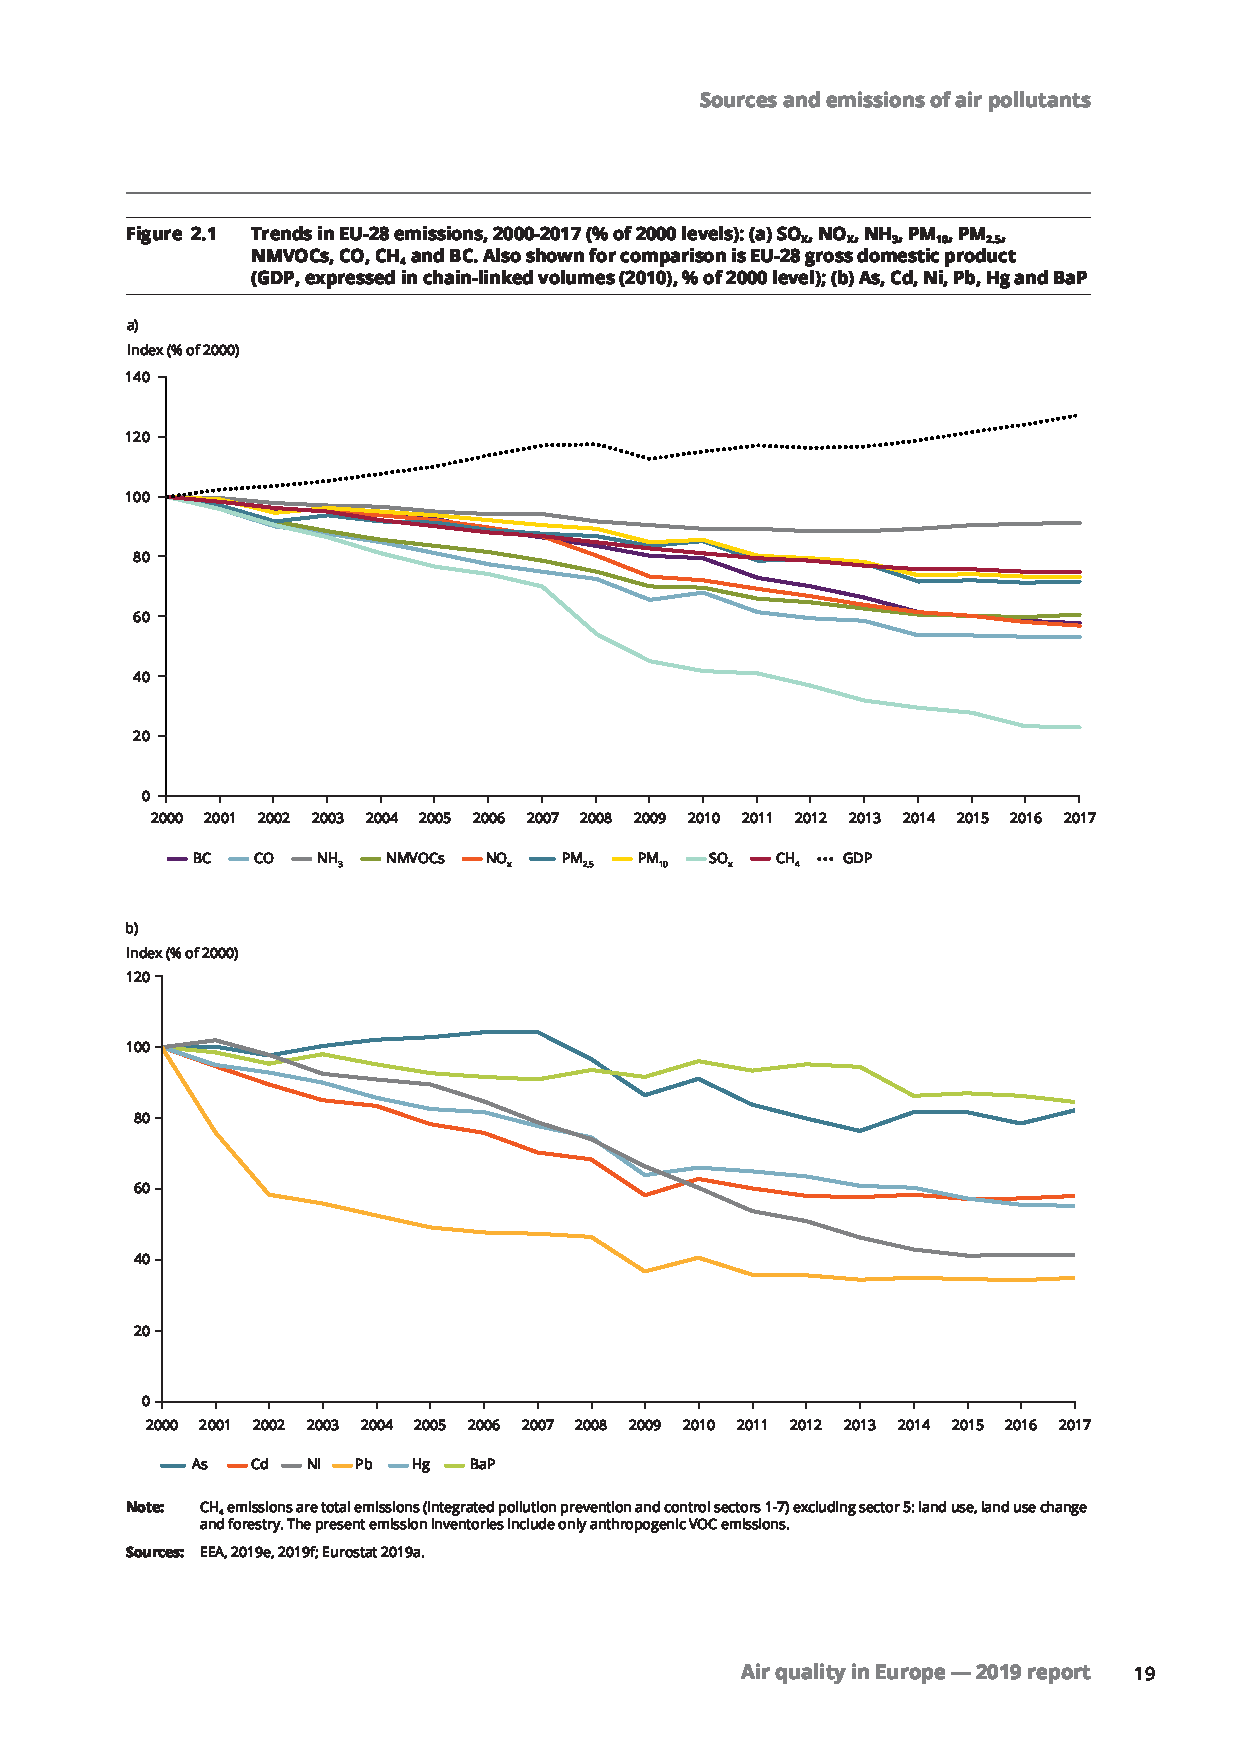
\includegraphics[clip,% left, bottom, right, top
        trim=0cm 15cm 0cm 5.8cm,%
        width=\textwidth]{img/pdf/european_emission_trends.pdf}
    \caption{General trends for European emissions. Data presented in \%
    emissions of year 2000. Note the downward global trend in pollutant
    emissions, and its decoupling with the European GDP~\cite{EEA2019}.}
    \label{fig:european_emission_trends}
\end{figure}

If one extends this analysis further, and separates emissions by using
their origin, the trends are approximately the same: except for
\gls{nh3} (a side product of agricultural activities) a clear reduction
is present in all sectors. These results can be seen in
Figure~\ref{fig:european_emissions_by_sector} and were presented
in~\cite{EEA2019}.

\begin{figure}[htpb]
    \centering
    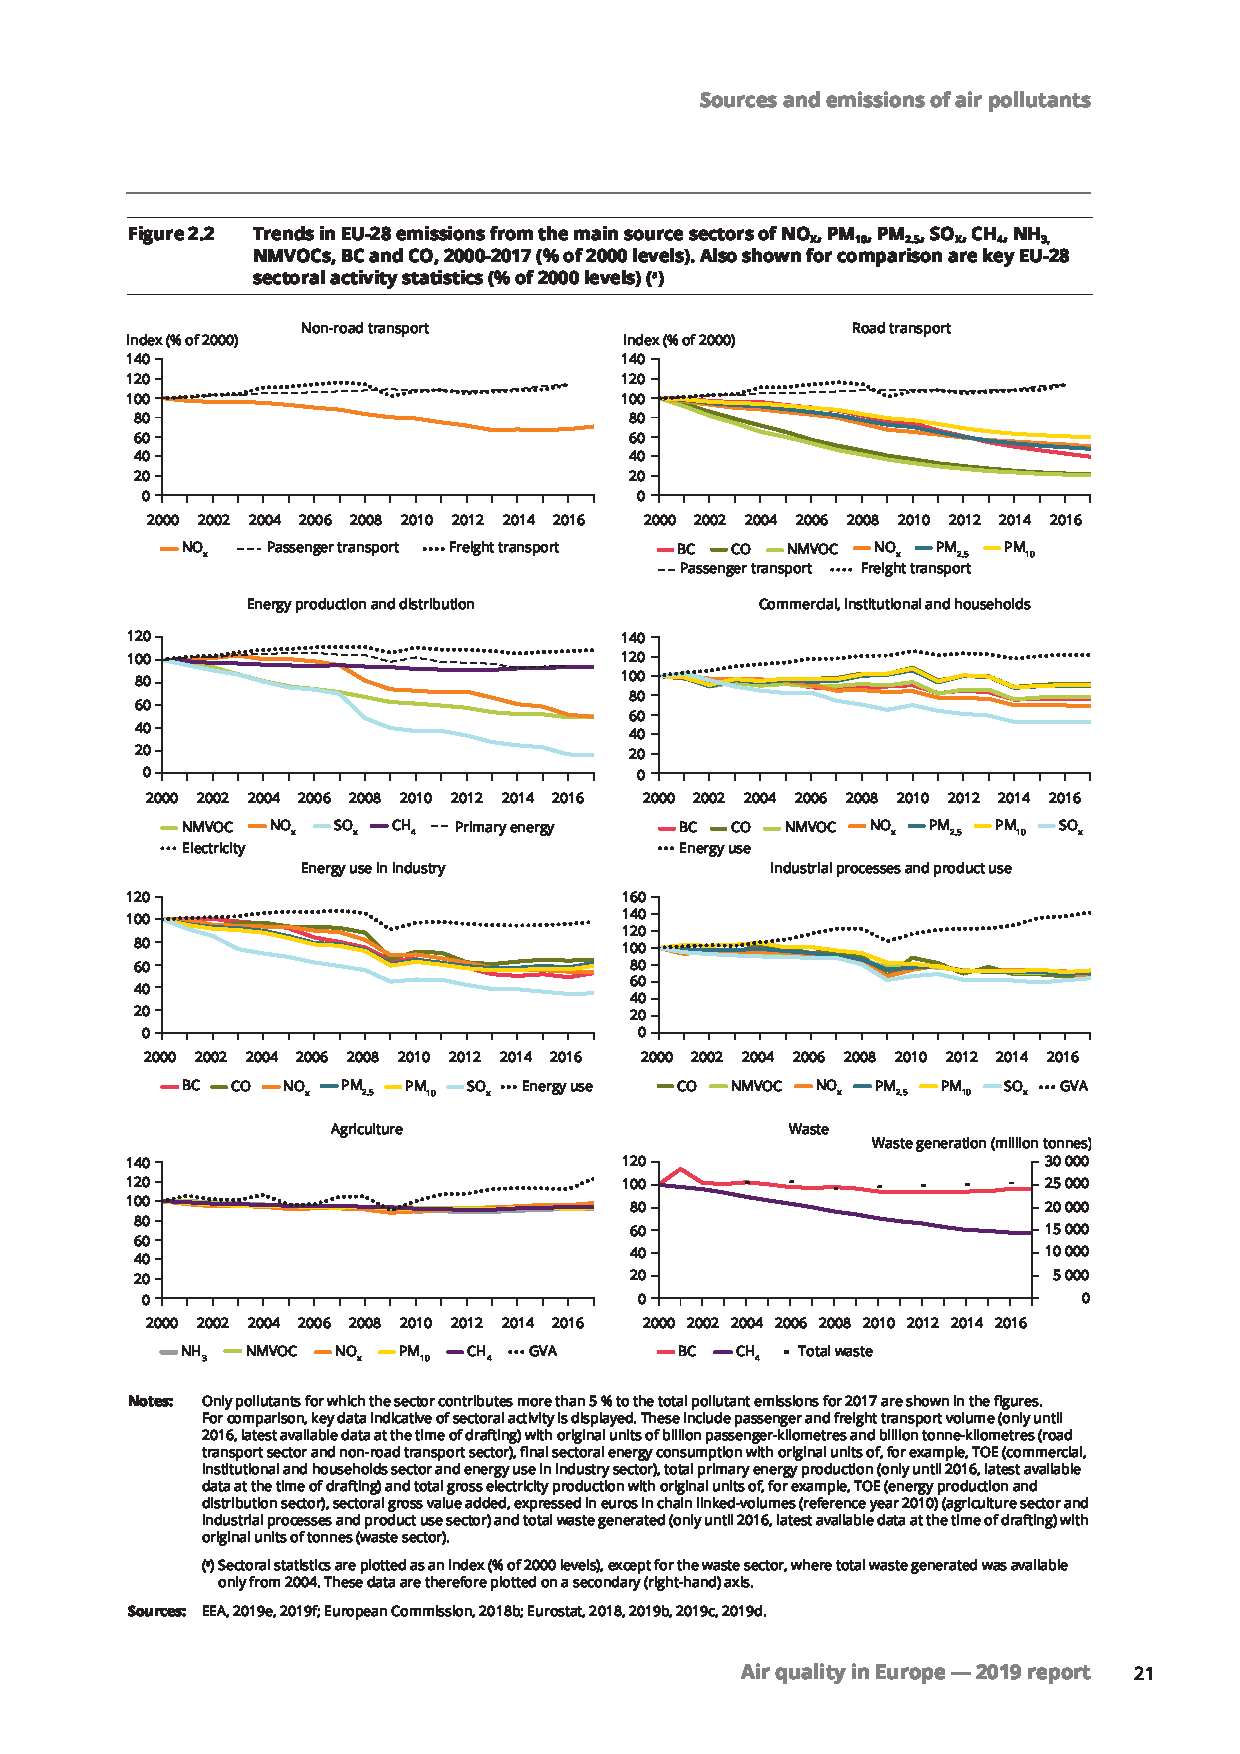
\includegraphics[clip,% left, bottom, right, top
        trim=0cm 6.5cm 0cm 5.3cm,%
        width=\textwidth]{img/pdf/european_emissions_by_sector.pdf}
    \caption{European emissions divided by activity sector. The global
    decreasing trend is confirmed, as industries all around are
    producing less and less \gls{AP} with the passing years~\cite{EEA2019}.}
    \label{fig:european_emissions_by_sector}
\end{figure}

\subsection{Detecting and Monitoring \acrlong{AP}}%
\label{sub:detecting_and_monitoring_ap}

There is no doubt that \gls{AP} is a global threat that affects
everyone, both in personal terms (through the degradation of their
health) and in societal terms, through the investments and limitations
that we as a whole have to commit to in order to prevent larger,
unmanageable problems. Reducing \gls{AP} is a priority and a requirement
for today's modern societies. This demands immediate and effective
actions, which in turn imply that we have a solid and profound
understanding of how pollutants are created, transported and transformed
in the atmosphere. The scale on which these interventions must be
conducted requires them to be made on a concerted and collaborative
manner, and always leveraged by technological
development~\cite{EEA2019}. Many of the air pollutants cannot be
detected solely by our senses, or even if they can is at already
dangerous concentrations. Technology is therefore a prerequisite to our
fighting the problem of \acrlong{AP}~\cite{Vallero2014}.

Pollution monitoring is itself based on the ability of a given
measurement method to determine concentrations for trace gases, aerosols
or radiation quantities. As with many other test techniques, in various
fields, pollution monitoring techniques have three very important
aspects to verify. The first of which is sensitivity, and also the most
demanding. Important trace gases in atmospheric chemistry have sometimes
vestigial concentrations, and the ability to correctly detect them is
many times a technical challenge. The second most important is
specificity, which is the ability of an atmospheric measurement to
measure each compound independently, without a component influencing
another component's measurement either positively or negatively.
Finally, any usable monitoring technique must be sufficiently precise as
to provide valid measurements.

There are literally dozens of methods for monitoring \gls{AP}, with
differing physical principles behind them. They can be categorized in
numerous ways, depending on the application and on the technique's
capabilities. Since it would be impossible to provide examples and
explanations for all possible methods, I will only present them for the
most commonly used techniques and for those that are related to this
thesis' spectroscopic method, \gls{DOAS}.



% \section{DOAS}%
% \label{sec:doas}

% \section{Tomography}%
% \label{sec:tomography}

\section{DOAS Tomography}%
\label{sec:doas_tomography}

%!TEX root=../slr.tex
\section{Introduction}
\label{sec:introduction}

% Contexto;
% Problema;
% Objectivos;
% Métodos;
% Resultados / contribuição;
% Conclusão;

This article comes as a response to the necessary State of the Art
search that was required for project ATMOS, which was a Portuguese EU
funded project that aimed to develop a miniaturised spectroscopy system
for atmospheric analysis and trace gas mapping using Differential
Optical Absorption Spectroscopy (DOAS), with tomographic capabilities.
FCT NOVA participated in this project as part of a consortium which also
included Compta, one of the oldest IT groups in Portugal. The project
aimed to develop a miniaturised and highly mobile spectroscopic system
with tomographic capabilities, designed to map a small geographic region
with respect to the concentration of a set of atmospheric trace gases,
like NO\textsubscript{2} or O\textsubscript{3}, using a technique called
Differential Optical Absorption Spectroscopy (DOAS).

DOAS is one of the most prominent methods for analysing and quantifying
atmospheric chemistry, namely in what concerns trace gas concentrations.
The technique, developed during the 70s by Perner and
Platt~\cite{Perner1976}, was popularised in the following decades by its
use in detecting Ozone, Nitrogen Oxydes and studies of cloud radiative
transport. DOAS is a type of absorption spectroscopy, which uses a
clever mathematical and physical observation to overcome the
difficulties of spectral measurement in the open atmosphere.

Through the setting of very careful geometric considerations, it is
possible to combine DOAS with tomographic reconstruction methods in
order to assemble a map of the gaseous concentrations in a given
geographic region. Tomography is the process of reconstructing an image
through projections obtained by subjecting a given target (in our case,
the atmosphere) to being traversed by any kind of penetrating or
reflecting wave, which in our case is visible light.

With this study, we have intended to capture the current literary
landscape surrounding the usage of tomographic DOAS, assessing this
technique's technological status. For this purpose, we have employed a
review methodology originary from Evidence Based Medicine. This method,
which has migrated to engineering through Software Engineering, is
called a Systematic Mapping Study (MS). It provides a framework that
allows researchers to produce detailed and systematic search protocols,
which are used to catalogue literature information and identify research
gaps within a determined subject.

The search procedure that we have defined was carefully engineered to
cover all tomographic DOAS research relevant to urban, rural or
industrial environments, with the main goal of finding a new
investigative path to follow. Through it, we were able to find several
different applications, all pertaining to scientific research, which are
similar regarding physical principle, but differ in objectives,
equipment assembly, algorithms, software, and geometry. Most of the
selected papers use an active DOAS principle for measuring atmospheric
chemical concentrations, and all of them are either fixed or of low
mobility. 

The rest of this paper has the following structure:
Section~\ref{sec:background} presents the context within which this
study was written; Section~\ref{sec:methods} describes how we have
planned to perform the study and the methods we have used in doing it;
Section~\ref{sec:conduction} describes the application of the said
methods in the pursuit of our goals and presents the results we have
obtained, as well as our evaluation of our processes;
Section~\ref{sec:conclusions} shows our conclusions and what we think
might be retained from reading this paper.

%!TEX root=../slr.tex
\section{Background}
\label{sec:background}

\subsection{Differential Optical Absorption Spectroscopy}
\label{ssub:differential_optical_absorption_spectroscopy}
Absorption Spectroscopy is the term used to identify all techniques that
use radiation absorption by matter to assess and quantify elements or
molecules in a given spectroscopic sample. It had, and still has, a very
important role in the study of the Earth's atmosphere~\cite{Platt2007}.

It is, as many other spectroscopic techniques, based on Lambert-Beer's
law, which states that 'in a medium of uniform transparency the light
remaining in a collimated beam is an exponential function of the length
of the path in the medium', as described originally by Pierre Bouguer in
1729, and can be written~\cite{Platt2007}:
\begin{equation}
    \centering
    I(\lambda) = I_0(\lambda) \cdot \exp[-L \cdot \sigma(\lambda) \cdot c]
    \label{eq:lambert_beer}   
\end{equation}

In Equation~\ref{eq:lambert_beer}, $I$ is the light intensity as measured by the
spectrometer, $I_0$ the original light intensity at the source, $L$ is
the optical path in which the sample is exposed to the light, $\sigma$
is the optical cross section of the sampled element or molecule and $c$
is the sample's concentration. $\lambda$ is the radiation's wavelength.

Lambert--Beer's equation, while valid in a laboratory setting, is
generally not enough to determine gaseous concentrations in an open
atmosphere experiment. $I_0$ determination would require require any
absorbant from the medium, which is impossible. Besides, in this medium,
there are many factors that influence measurements: Rayleigh's
scattering, Mie's scattering, thermal variations, turbulence and
instrumental transmissivities. All these play an important part in
altering atmospheric light~\cite{Platt2007, Merlaud2013}.

Differential Optical Absorption Spectroscopy (DOAS) overcomes these
difficulties by capitalising on cross section's differences between
interfering phenomena (normally broad spectral features) and certain
trace gases (usually narrow spectral structure).  The mathematical
formulations behind the technique are well beyond the scope of this
article, but suffice it to say that the broad structures are removed
through subtraction of a fitted low order polynomial, and a fitting
algorithm (such as Levenberg-Marquardt) is used to retrieve
concentrations. Detailed presentations of these procedures are presented
in~\cite{Platt2007} and~\cite{Merlaud2013}.

In~\cite{Platt2007}, the authors split the DOAS method into two
fundamental families: passive and active. The passive family is
characterised by being designed to capture and analyse natural light,
whether from the Sun, the Moon or any other celestial body. This kind of
measurement has the advantage of being simple to assemble, but natural
light usage implies an additional technical effort for the retrieval of
atmospheric concentrations. Active DOAS applications, on the other hand,
use artificial light sources to make their measurements. This has been
used extensively in the identification of several atmospheric
components. Its concentration extraction procedure is simpler, at the
expense of a more complex assembly.

DOAS has had a number of applications throughout the years. The
technique was first applied in the 1970s. At that time, Perner used an
active setup with a laser light source to identify the OH radical in the
atmosphere~\cite{Perner1976}. More recently, researchers around the
world have been employing broadband sources (such as Xenon lamps) to
measure trace gases like Ozone, Nitrogen Dioxide or Sulphur Dioxide.
Almost simultaneously, passive systems have been used to study
stratospheric chemistry and radiative transport in
clouds~\cite{Platt2007}.

\subsection{Multi-Axis DOAS}%
\label{sub:multi_axis_doas}

Multi-Axis DOAS (MAX-DOAS) is one of the more recent applications of the
DOAS technique. It represents a significant progress regarding zenith
scattered sunlight measurements, a well established atmospheric analysis
technique. It performs a series of passive DOAS measurements in several
telescope elevations (typically 4 to 10)~\cite{Honninger2004}, either in
sequence or simultaneously, according to the schematic representation in
Figure~\ref{fig:max_doas}. 

\begin{figure}[htpb]
    \centering
    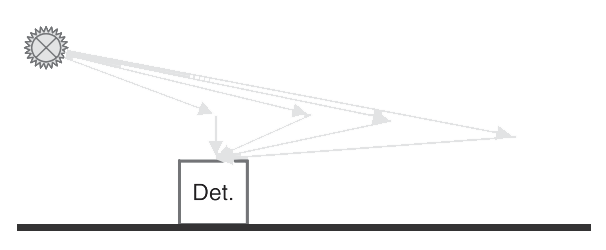
\includegraphics[width=0.8\linewidth]{img/maxdoas.png}
    \caption{MAX-DOAS schematic representation~\cite{Platt2007}.}
    \label{fig:max_doas}
\end{figure}

MAX-DOAS stems from another set of techniques called \emph{off-axis},
which in this case means that the telescope is pointed at another angle
than the zenith. Off-axis DOAS was first employed in 1993 when Sanders
et al.~\cite{Sanders1993} used it to assess OClO in Antarctica. During this
experiment, the team concluded that the off-axis geometry greatly
improves sensitivity for tropospheric species, but does not change the
system's ability to quantify stratospheric absorbers.

By evaluating several directions, the technique allows researchers to
measure not only stratospheric contributors, as zenith sky assemblies,
but also to detect absorbers at ground level, as an active DOAS
instrument would.

We mention MAX-DOAS in this paper because one could argue that these
systems would be able to be adapted to perform tomographic measurements,
if more than one system would analyse the same region from more the same
number of observation angles. MAX-DOAS tomography is a special case, and
would probably deserve to be investigated fully. However, since this was
not the object of our study, we chose not to specifically target this
method in our search.

\subsection{Imaging DOAS}%
\label{sub:imaging_doas}

Imaging DOAS combines spectral and spatial information by combining an
imaging spectrometer with a scanning system. The resulting data clearly
resembles that of a hyperspectrum, as Figure~\ref{fig:idoas_results}
illustrates.

\begin{figure}[htpb]
    \centering
    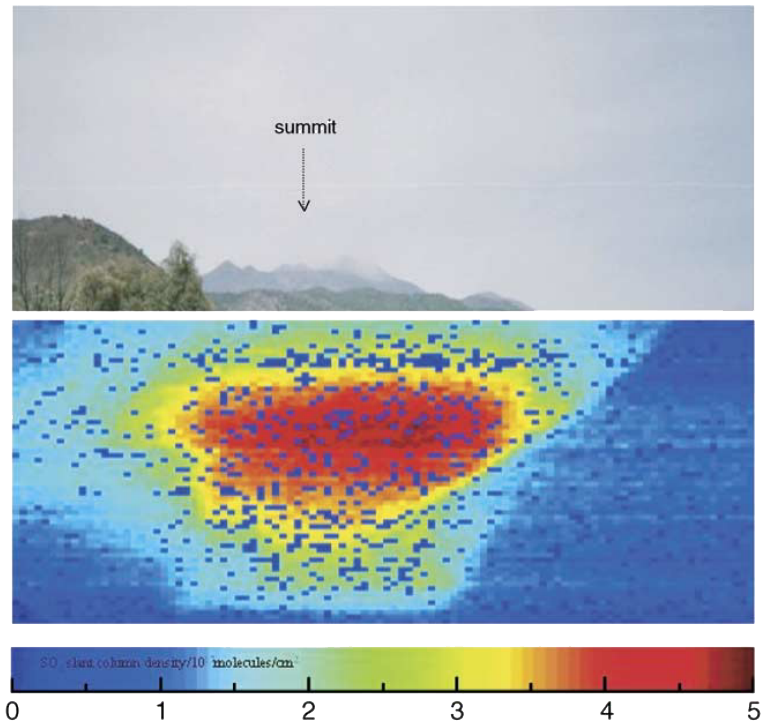
\includegraphics[width=0.5\linewidth]{img/idoas_results.png}
    \caption{IDOAS results over mount Etna, in Italy. The colour coded
    map under the digital photograph represents the SO$_2$
concentration~\cite{Bobrowski2006}.}
\label{fig:idoas_results}
\end{figure}

The method, developed by Bobrowsky et al.~\cite{Bobrowski2006}, employs a 2D
CCD detector. One dimension measures spectral information, while the
other contains spatial information for one direction. The other spatial
direction is obtained by scanning the field of view with the pushbroom
method. A schematic representation is presented in the same article, and
is here reproduced in Figure~\ref{fig:idoas_schematic}.

\begin{figure}[htpb]
    \centering
    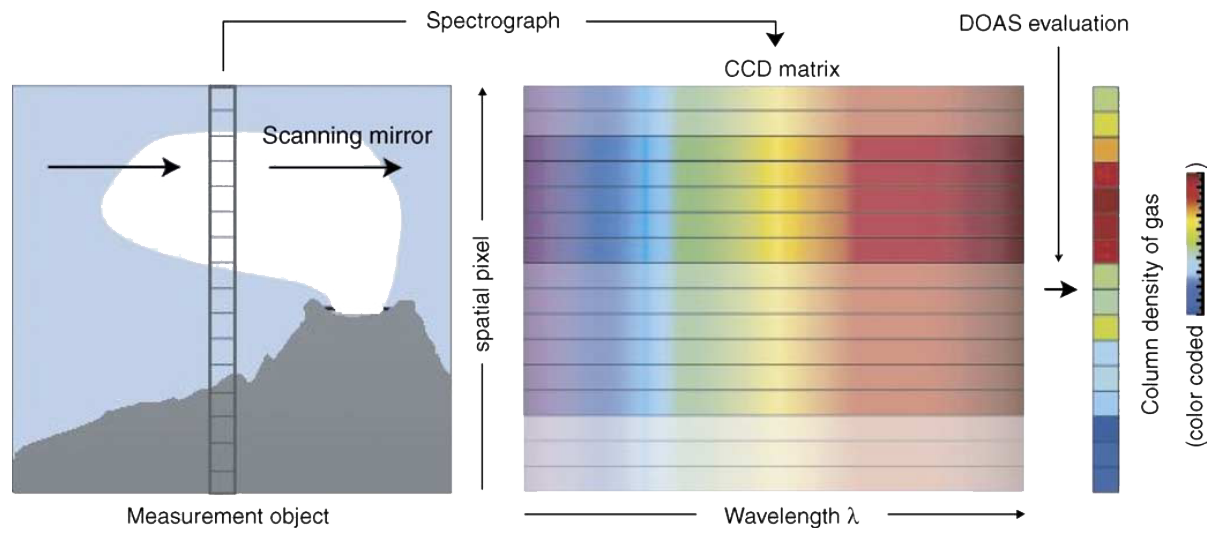
\includegraphics[width=0.8\linewidth]{img/idoas_schematic.png}
    \caption{IDOAS capture functioning schematic ~\cite{Bobrowski2006}.}
    \label{fig:idoas_schematic}
\end{figure}

DOAS is used to yield slant column density values for the absorbers for
each pixel. The values are colour coded and produce an image describing
the gas distribution.

This technique is included in this paper because it exists in order to
produce a two-dimensional image from spectral information. This image,
however, does not come from a tomographic reconstruction procedure, nor
is spatial information recovered from projections, but instead comes
directly from the acquisition method. Hence, we did not include articles
on this method in this study.
% END DOAS

\subsection{Tomography}
\label{sub:tomography}
Tomography refers to the set of techniques that aim to produce a cross
sectioning image from data collected by exposing a given target body to
some kind of penetrating or reflecting wave from many different
directions~\cite{Herman2009, Kak2001a}.

The initial theories that gave rise to tomography were laid out by
Johannes Radon in 1917, with a mathematical operation that  would later
be known as the Radon transform. This process maps a function f, defined
in the plane, to the function Rf, comprised of the values of the line
integrals of f, taken in $\theta$ directions. In practice, this
formulation allows the reconstruction of an image by its projections,
which are nothing more than line integrals~\cite{Feeman2010}.

Tomographic image reconstruction can be achieved by running one of
several algorithms through a computer program. The presentation of these
algorithms is completely beyond the scope of this article, but a good
starting point for learning about these operations is \emph{The
Mathematics of Medical Imaging}, by Timothy Feeman~\cite{Feeman2010}. It
is in the scope of this article, however, to make a small introduction
to a particular set of reconstruction methods. The reason for this being
the prevalence of these methods in the field of DOAS tomography, which
is the main subject of this study. These techniques are thus:
\begin{description}
    \item[Algebric Reconstruction Techniques (ART)] Proposed in 1970 by
        Gordon and Herman~\cite{Herman1973}, these techniques are based
        on successive approximations between the actual projection data
        and the sum of the reconstruction elements which represent
        it~\cite{Gordon1974}. The process is conducted line by line,
        until a satisfactory convergence condition is met.

    \item[Simultaneous ART] Simultaneous ART is very similar to the ART
        algorithm. The difference being that the iterative changes occur
        for all lines at the same time, instead of in only one.

    \item[Simultaneous Iterative Reconstruction Techniques (SIRT)] The
        main difference between SIRT and SART is that in the former,
        cell changes are not reflected immediately after one
        calculation. Updates occur at the end of each iteration. At this
        point, the change for each cell is the average correction
        calculated for it taking all equations into
        account~\cite{Kak2001}.
\end{description}

During the second half of the twentieth century, tomographic processes
have had a revolutionary influence in many fields of study, but
especially in medicine (see Figure~\ref{fig:ct_scan}). Computational
tomography scanners allow doctors to see their patients interior in a
highly detailed and extremely safe fashion. At first, tomographic
imaging was performed only with X-Rays.  Their attenuation throughout
the patient's body being used as a projection. Nowadays, there are much
more methods of image retrieval, such as radioisotopes, ultrasound or
particle anihilation~\cite{Kak2001a, Feeman2010, Herman2009}.

\begin{figure}[htb]
    \centering
    % \includegraphics[width=0.8\linewidth]{ct_scan.png}
    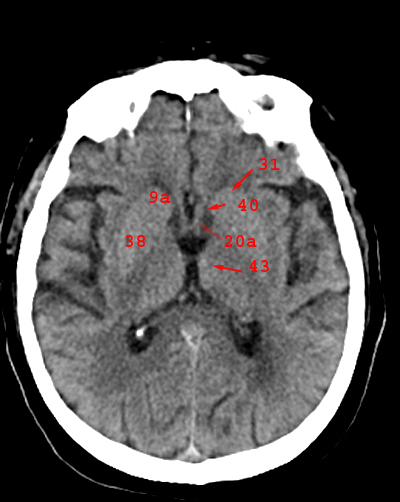
\includegraphics[width=0.6\textwidth]{img/CT07.jpg}    
    \caption{Tomographic image, axial view of the human
        brain~\cite{Glowniak}. Note how a trained clinician can identify
        several structures (7 red notes) with just one slice of a
        computerised tomography image. Before tomographic techniques
        were invented, it was impossible to retrieve this this kind of
        detail without dissecting the patient.}
    \label{fig:ct_scan}
\end{figure}

Although it was the field of medicine was more influenced by tomographic
procedures than any other, the applications of these methods are not
restricted to it. One can find numerous industrial and research
applications~\cite{Wang2015, Haisch2012, Byer1979}. One of which is the
application to atmospheric research, namely in conjunction with DOAS. In
recent years, scientists have been working on tomographic methods for
measuring atmospheric trace gas concentration values. The field is
interesting because it allows for 2D or even 3D mapping of a given
region, with respect to those trace gases. This article aims to make an
assessment of the status of this tomographic application, by analysing
current literature on the subject. 
%END TOMOGRAPHY



\subsection{Mapping Study}
\label{sub:mapping_study}

A Systematic Mapping Study (MS) is a type of secondary study designed to
determine the general features of the research landscape in the subject
they are addressing~\cite{Kitchenham2007, Petersen2008}.

An MS is driven by broad (and often multiple) research questions and
applies an also broad data extraction protocol. This is in line with the
fact that this kind of study aims to summarise its findings, answering
the research questions, and in-depth analysis is not required. It is
common for an MS to be a precursor to a Systematic Literature Review
(SLR), which is a much deeper kind of systematic study. Guidelines for
performing studies of both kinds can be found in a report made by
Kitchenham and Charters in 2007~\cite{Kitchenham2007}. In this document,
the authors establish the 3 stages which all MS and SLR generally have:

\begin{description}
    \item[Planning] This stage includes all preliminary considerations
        regading the MS or SLR in the making. All protocols, from search
        to evaluation, through data extraction, are devised;
    \item[Conduction] During this staged, researchers apply what they
        have planned in the previous phase. Protocols are
        \emph{actually} run, and data is synthesised;
    \item[Reporting] In this phase, the team has to define their
        dissemination strategy, and implement it. It is in this stage
        that a final report is written and evaluated.
\end{description}

Although it is logical (and fundamentally correct) to assume that these
steps are sequential, this may not be, and usually is not, accurate.
Many of these stages and their intermediate steps require iteration. For
instance, some inclusion or exclusion criteria may only be found
necessary once the search protocol is implemented.

% End Mapping Study
%\subsection{Methods}
%\label{sub:methods}

%Given our goals and the particular methodology that we have chosen to
%adopt with this study, it is important to provide a small introduction
%to how we have planned to proceed and what we will be evaluating.

%\subsection{Research Questions}
%\label{sub:research_questions}

%As stated in Kitchenham's 2007 report~\cite{Kitchenham2007}, Research
%Questions (RQ) are what drives every MS. There are several types of
%research question. They can be focused on costs, advantages or
%assessment of a given technology or procedure. In our case, we are more
%interested in this latter type. The literature on SLR and MS recommend
%establishing RQs by considering them through some standard viewpoints, a
%guideline that is refered to as a PICOC analysis:

%\begin{description}
%    \item[Population] the ones affected by the study or the technology
%        that is being assessed;
%    \item[Intervention] the specific methodology or tool which will be
%        applied to the subject of interest, with the MS goals in mind;
%    \item[Comparison] a benchmark with which to compare obtained
%        results;
%    \item[Outcomes] the expected results of the MS or SLR study in
%        question.
%\end{description}

%A more profound analysis of how our RQ are defined can be found in
%Section~\ref{sec:methods}, but since our goal is to map research
%literature on the subject of DOAS tomography, our main research question
%is \textbf{\emph{What is the current status of the technology used in
%tomographic DOAS?}}.
%% End of Research Questions

%\subsection{Data Extraction Strategy}
%\label{sub:data_extraction_strategy}

%After having defined the RQ, it is important to plan how the study will
%try to answer those questions. This is to say a \emph{data extraction
%strategy}. It includes the choice of libraries, the definition of a
%search string, exclusion and inclusion filters,  and the scoring method
%for each article. It also includes the description of how the data is to
%be assessed within each paper. 

%Section~\ref{sec:methods} includes a complete description of how this is
%approached, while a summarised presentation of how we have approached
%this is illustrated in Table~\ref{tab:data_extraction_summary}.

%\begin{table}[htb]
%    \centering
%    \caption{Data extraction: a small summary.}
%    \label{tab:data_extraction_summary}
%    \begin{small}
%        \begin{tabular}{@{}ll@{}}
%        \toprule
%        \multirow{5}{*}{\textbf{Libraries Searched}} & Google Scholar\\
%                                                    & IEEE\\
%                                                    & Web of Knowledge\\
%                                                    & Science Direct\\
%                                                    & American Geophysical Union\\ \midrule
%        \textbf{Search String}                      & DOAS atmospher* tomography                \\ \midrule
%        \multirow{5}{*}{\textbf{Exclusion Filters}} & Duplicate in Scholar                      \\
%                                                    & Non English articles are not accepted     \\
%                                                    & Satellite data papers are not accepted    \\
%                                                    & Volcanology papers are not accepted       \\
%                                                    & CNKI published articles are not accepted  \\ \midrule
%        \multirow{2}{*}{\textbf{Inclusion Filters}} & Must be full articles                     \\
%                                                    & Must be about Tomographic DOAS            \\ \midrule
%        \textbf{Papers found}                       & 732                                       \\ \midrule
%        \textbf{Papers discarded}                   & 724                                       \\ \midrule
%        \multirow{2}{*}{\textbf{Screening methods}} & 1. Abstract analysis to produce shortlist \\
%                                                    & 2. Full read of shortlisted articles      \\ \midrule
%        \textbf{Analysed papers}                    & 8                                         \\ \bottomrule
%        \end{tabular}    
%    \end{small}
%\end{table}
%%End of Libraries
%%End of Methods

%\subsection{Results}
%\label{sub:results}

%As can be seen in Table~\ref{tab:data_extraction_summary}, our search
%returned around 730 results, of which a small fraction (8) managed to
%pass all exclusion and inclusion filters we had defined. With reference
%to the structure of the retrieved results, it is important to note that
%most of the results (80\%) came from Google Scholar.

%As to the analysis, we have found that instrument descriptions were
%found in 6/8 articles; algorithm descriptions in 5/8 articles, and
%software mentions in 3/8 articles. We have also found that there were
%5/8 empirical papers (associated to an experiment) while the
%remaining 3/8 were theoretical papers. Following our scoring method
%(defined in Table~\ref{tab:quality_assessment_criteria}), our 8 articles
%had achieved an average score of 0,48, with a median of 0,6. Although
%the sample is very small, this disparity between average and median
%hints at the existence of outliers or some kind of clustering.

%As to the setup information that we have set out to obtain, we were able
%to extract several instrument configurations, algorithms and used
%software, which are presented and discussed in
%Section~\ref{sec:conduction}. 
%%End of Results

%\subsection{Conclusions}
%\label{sub:conclusions}

%DOAS tomography has many possible applications and many possible
%interested parties. However, literature on the subject, especially in
%what refers to urban, rural or industrial scenarios is limited. The
%technology used for the different systems surveyed in this study is
%mostly the same active DOAS setup, granted some peculiarities of each
%system. The method is also very research-focused, although some
%researchers seem to be near a commercial/industrial application.

%%End of Conclusions

%!TEX root=../slr.tex

\section{Methods}\label{sec:methods}

In the elaboration of this article, we took the three normal stages of
SLR conduction: planning, conduction and reporting. The first stage
involves making the decisions that guide the rest of the process; the
conduction phase is comprised of the actual gathering of data, using the
protocol defined in the first stage. The final section of the study is
basically the writing and the publishing of the results. In this
section, we present the methods used in the study and their rationale,
which roughly corresponds to the planning stage.

\subsection{Objectives}
\label{sub:objectives}

An MS always aims to answer its research questions in a broad but
definite way. It is a way of understanding a given field of research,
and being able to systematise how this understanding is achieved.

As stated before, this is an MS aimed at characterising DOAS tomography
general status. In doing this, we pretend to get a clearer image of what
has been done and what should be attempted next, hopefully managing a
sort of roadmap for future research contributions.
%End Objectives

\subsection{Research Questions}
\label{sub:research_questions_and_search_queries}

We have begun by defining the goals for our study, and structuring them
with a PICOC (Population, Intervention, Context, Outcome and Comparison)
analysis, which is summarised in Table~\ref{tab:picoc}. This analysis
led us to our research goal: \textit{to assess the technological status
    of the DOAS tomography technique}.
    
We used this goal statement as a primer to our research question,
which was then formulated as: \textbf{what is the current status of
the technology used in tomographic DOAS?}

\begin{table}[htb]
\small
\centering
\caption{PICOC analysis.}
\label{tab:picoc}
\begin{tabular}{@{}ll@{}}
\toprule
\textbf{Population} & DOAS research in general.\\ 
\textbf{Intervention} & The papers must address tomographic DOAS.\\
\textbf{Outcome} & Status \textbf{assessment} for \textbf{DOAS tomography}.\\
\textbf{Context} & Research papers.\\\bottomrule
\end{tabular}
\end{table}

Now, this question is too vague to pursue in a systematic fashion, so we
had to slice it into smaller and more objective chunks. This sectioning
is presented in Table~\ref{tab:rq_slicing}.

\begin{table}[htb]
\centering
\small
\caption{Research question slicing}
\label{tab:rq_slicing}
    \begin{tabularx}{\textwidth}{lX}
        \toprule
        \textbf{Original} & What is the current status of the technology used in
        tomographic DOAS? \\
        \textbf{RQ1} & Is there a typical hardware setup used in tomographic
        DOAS studies? \\
        \textbf{RQ2} & Is there a standard software used to perform these
        analysis? \\
        \textbf{RQ3} & What are the algorithms more commonly used?\\\bottomrule
    \end{tabularx}
\end{table}

The research question is one of the most important steps in planning a
Systematic Literature Review, but it cannot be entered into a library's
search box. Therefore, we have to define our search terms before we can
make any effort of answering our questions.

\subsection{Search Query Definition, Library Selection and Filter Definition}
\label{sub:library_selection_and_filter_definition}

In the case of this study, the search terms were selected in order to
purposefuly maintain a broad scope, so that we could retrieve a high
number of relevant studies. The selected search terms were: \textbf{DOAS
atmospher* tomography}\footnote{The asterisk acts as a wildcard.}. The
search query was entered into 5 academic search engines, as shown in
Table~\ref{tab:libraries}.

\begin{table}[htb]
\centering
\caption{Electronic libraries used in this study.}
\label{tab:libraries}
\begin{tabularx}{\textwidth}{ll}
\toprule
\textbf{Library}          & \textbf{URL}\\
\midrule
Google Scholar (GS)   & https://scholar.google.com/\\
Web of Knowledge (WoK)& https://webofknowledge.com\\
Science Direct (SD)   & https://www.sciencedirect.com\\
IEEE             & http://ieeexplore.ieee.org/\\
AGU Publications (AGU) & http://agupubs.onlinelibrary.wiley.com/hub/\\
\bottomrule
\end{tabularx}
\end{table}

After setting Table~\ref{tab:libraries} libraries, it was time to define
our article selection criteria, which are summarised in
Table~\ref{tab:select_filters}. We began with 2 Inclusion Criteria (IC)
and 3 Exclusion Criteria. The IC determined that our selected papers
would have to be journal articles (thus exluding thesis, white papers,
patents and other documents) and that these articles should be on the
topic of Tomographic DOAS. The EC dictated that no selected paper should
include volcanology studies or satellite data analysis (these have
particularities which we do not want to approach in this study) and that
no other language than English will be accepted.

During the course of the search, however, we had to include another two
EC. The first was included in the Google Scholar search, where we
understood that papers from a certain publisher were not accessible. The
second came in the subsequent searches, when it became clear that most
papers had already been retrieved by the GS search. 

\begin{table}[htb]
\centering
\caption{Selection filters in use for this study's search.}
\label{tab:select_filters}
\begin{tabularx}{\textwidth}{lXl}%{@{}cll@{}}
\toprule
\multicolumn{1}{l}{} & \textbf{Criterium} & \textbf{Definition} \\ \midrule
\multirow{5}{*}{\textbf{Exc. Criteria}} & EC1 & Duplicate in Scholar \\
 & EC2 & Non English articles are not accepted \\
 & EC3 & Volcanology papers are not accepted \\
 & EC4 & Satellite data papers are not accepted \\
 & EC5 & CNKI published articles are not accepted \\ \midrule
\multicolumn{1}{l}{\multirow{2}{*}{\textbf{Inc. Criteria}}} & IC1 & Results must be articles \\
\multicolumn{1}{l}{} & IC2 & Results must be about Tomographic DOAS \\ \bottomrule
\end{tabularx}
\end{table}

\subsection{Data Extraction Strategy}
\label{sub:data_extraction_strategy}

The data extraction process is a key part of any systematic review,
whether an SLR or an MS. It determines how each article is approached
with regard to its content, before any information is retrieved. In our
case, our strategy took place in two separate moments: an initial
screening, in which we would assess contents as expressed by the
articles' abstract; and a second moment, in which we performed a full
article read. Special attention was given to explicit sections covering
our target topics (equipment, algorithm and software). 

% End of data extraction strategy

\subsection{Quality Assessment}
\label{sub:quality_assessment}

It is very difficult to assess a paper's quality, and to rank it
accordingly. However, for this review in particular, we have decided to
follow Souza's approach~\cite{Souza2019} and adopt a similar evaluation
method.  Table~\ref{tab:quality_assessment_criteria} contains the used
criteria. 

In our evaluation model, we took into account both general ans specific
criteria. The former addresses an article's contributions to our
particular SLR; the latter targets the actual content of that article. 

In order to measure the contribution of each individual paper to our
study (our general criterium), we have assessed its number of citations
in all the other selected papers. This is a valid measurement of a
papers impact in the study, but it might become difficult to implement
if a high number of articles are selected for the final stage.
Contentwise (specific criteria), we have defined our scoring model
according to the Research Question separation explained in
Subsection~\ref{sub:research_questions_and_search_queries}.

\begin{table}
    \centering
    \caption{Quality assessment criteria presentation.}
    \label{tab:quality_assessment_criteria}
        \begin{small}
            \begin{tabularx}{\textwidth}{lXXr}%{@{}llll@{}}
                \textbf{Criterium Type} & \textbf{Criterium (Weight)} & \textbf{Decision Factor} & \textbf{Score} \\ \midrule
                \multirow{4}{*}{\textbf{General Criteria}} &
                \multirow{4}{*}{Contribution to this SLR (0,2)} & cited in study: more than three times & 1 \\
                 &  & cited in study: three times & 0,75 \\
                 &  & cited in study: twice & 0,5 \\
                 &  & cited in study: once or less & 0,25 \\ \midrule
                \multicolumn{1}{l}{\multirow{10}{*}{\textbf{Specific Criteria}}}
                & \multirow{4}{*}{Algorithm description (0,6)} & Detailed & 1 \\
                \multicolumn{1}{l}{} &  & Semi-Detailed & 0,4 \\
                \multicolumn{1}{l}{} &  & Mentioned & 0,2 \\
                \multicolumn{1}{l}{} &  & None & 0 \\ \cmidrule(l){2-4} 
                \multicolumn{1}{l}{} &
                \multicolumn{1}{c}{\multirow{4}{*}{Instrument description (0,2)}} & Detailed & 1 \\
                \multicolumn{1}{l}{} & \multicolumn{1}{c}{} & Semi-Detailed & 0,4 \\
                \multicolumn{1}{l}{} & \multicolumn{1}{c}{} & Mentioned & 0,2 \\
                \multicolumn{1}{l}{} & \multicolumn{1}{c}{} & None & 0 \\ \cmidrule(l){2-4} 
                \multicolumn{1}{l}{} & \multirow{2}{*}{Software Description (0,1)} & Mentioned & 1 \\
                \multicolumn{1}{l}{} &  & None & 0 \\ \bottomrule
            \end{tabularx}    
        \end{small}
    
\end{table}

In our study's case, distinction between Specific and General was not
sufficient to adequately separate scores according to importance. It was
necessary to introduce scoring weights for that end. These weights are
also shown in Table~\ref{tab:quality_assessment_criteria} and were set
according to the goals of our SLR, meaning that the tomographic element
is the most important.

In the end, a paper's total score comes from the formula described by
Equation~\ref{eq:score}.

\begin{equation}
    \centering
    \label{eq:score}
    Total Score = \sum_{i} w_{i} \cdot S_{i}
\end{equation}

Where $S_i$ and $w_i$ are a paper's score and weight for a given
criterium, respectively.

Finally, we shall discuss the different weights given to each criterium
and the different ways in which they are evaluated. The most important
aspect that we are trying to assess is the algorithm, which defines the
whole tomographic process and the results achievable by the studies.

A detailed algorithmic description includes the mathematical basis as
well as a complete description of required adaptations, both on the
mathematical level and on a conceptual method.

Instrument description is also an important criterium, since it is with
it that scientists retrieve the information they will afterwards process
tomographically, through the algorithm.

It is sometimes difficult to establish how good an instrument descrition
is. A too detailed description can be just as bad as a non-sufficient
one, if the equipment options are not correctly presented.

That being said, we have considered a detailed description one that
includes explicit mention to the composition of the optical system and
its assembly details, together with the analysing hardware (e.g.
spectrometers) configuration and capabilities.

The least important of the technical features under evaluation is the
software. This is because theoretically, results would be the same
independently of the software in use. We have included this feature in
the study as a way of identifying if there was some kind of software
prevalence in the community. In this study, software is binarily
assessed: either the scrutinised study mentions it or not.

Finally, we evaluate the contribution of each article to this study.
Since DOAS tomography is a field with a relatively low number of
players, it can be expected that there are many cross citations. We have
introduced this as a method of measuring an article's relative
importance within this mapping study, simply by counting the number of
times a cross citation occurs.

%!TEX root=../template.tex

\section{Conduction}
\label{sec:conduction}
\subsection{The Search}
\label{sub:the_search}

SLR guideline literature \cite{Kitchenham2007,Tacconelli2010} recommend
that the first stage of any Systematic Literature Review or Mapping
Study be the search for previous literature of this kind, since a recent
systematic study may render the execution of a new study
disencourageable. In our case, none of the several libraries used
appeared to have any article of the sort.

The search terms, derived in
Subsection~\ref{sub:research_questions_and_search_queries}, were run in
all libraries found in
Subsection~\ref{sub:library_selection_and_filter_definition}. The Google
Scholar search had the particularity of being run through a specialised
software called \textit{Publish or Perish}\cite{Harzing}, which allowed
the search results to be exported to a comma separated values file,
which made the process a lot easier, since it was then possible to work
the data directly in a spreadsheet program (Microsoft Excel, in this
particular case).

The conduction phase of our study followed the flowchart illustrated by
Figure~\ref{fig:flowchart}. Notice that Google Scholar is the first
library to be searched. This is motivated by the fact that the vast
majority of the articles were retrieved by Google's academic search
engine. In fact, GS-retrieved articles were so predominant that we had
to create a special EC, as described in
Subsection~\ref{sub:library_selection_and_filter_definition}.

\begin{figure}[htpb]
    \centering
    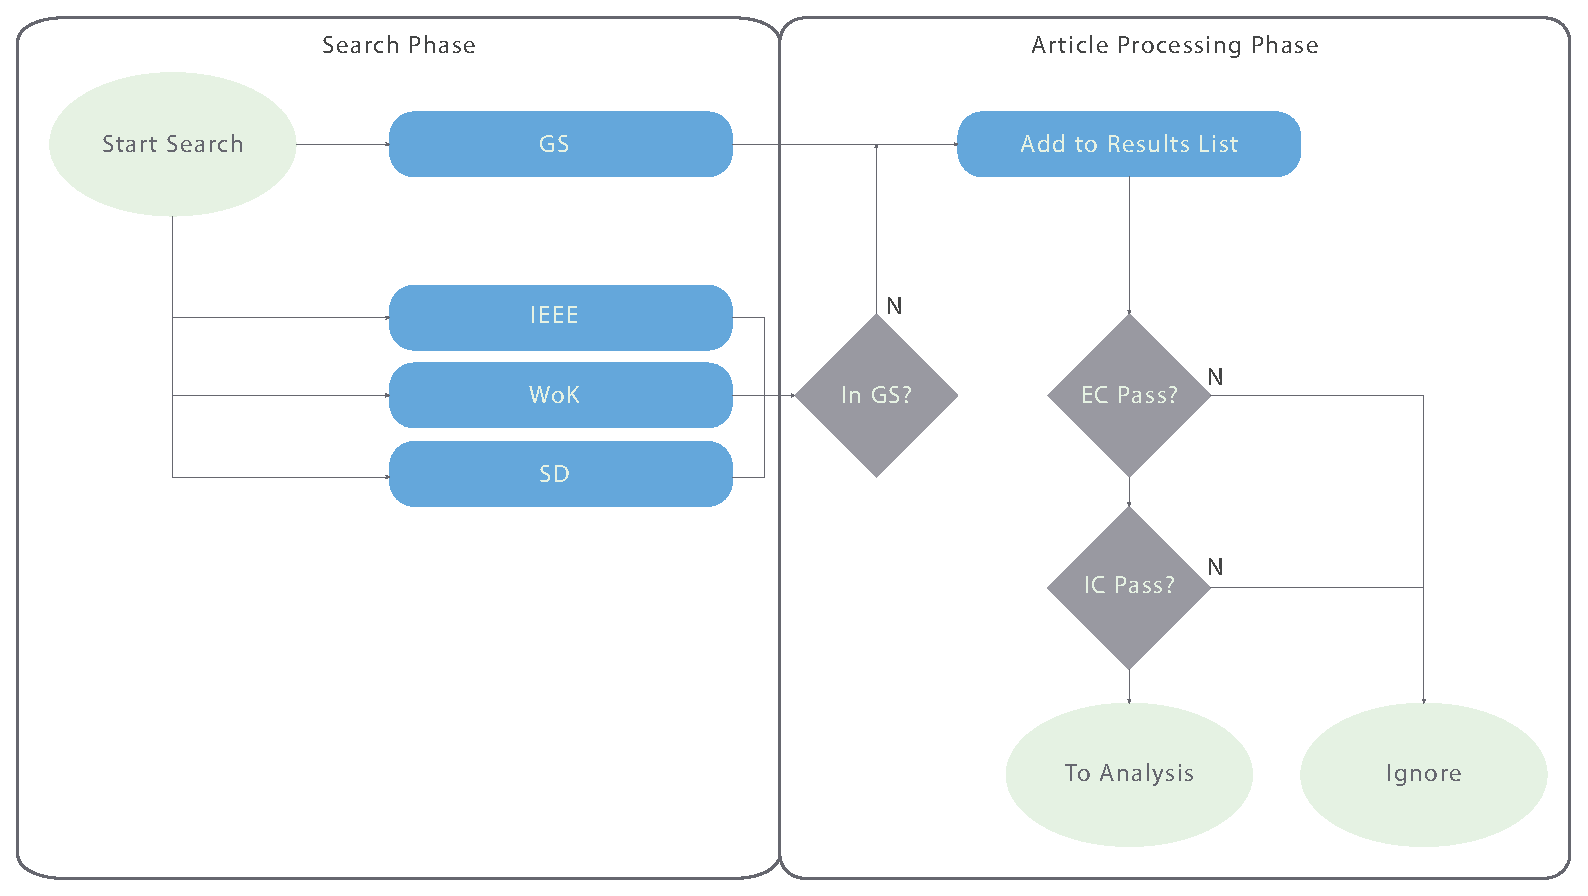
\includegraphics[width=\linewidth]{img/flowchart.eps}
    \caption{Conduction stage flowchart. Notice Google Scholar's
    prevalence.}
    \label{fig:flowchart}
\end{figure}

\subsection{Results and Discussion}
\label{sub:results_and_discussion}

\subsubsection{Presentation and analysis}
\label{ssub:result_presentation}

Our search returned 732 results, of which 709 were distinct
($\approx$97\%). Of these, 601 were journal articles ($\approx$82\%).
The vast majority of the results came from GS ($\approx$80\%, see
Figure~\ref{fig:results_distribution}).  Selection criteria (Inclusion
and Exclusion) application resulted in the exclusion of 701 results
($\approx$99\%), thus leaving 8 articles reaching the content analysis
stage (the attempt to answer the Research Question). A summary of these
findings can be seen in Table~\ref{tab:search_results}.

 \begin{table}[htb]
    \centering
    \caption{Search results. For a paper to reach the righmost column,
    which means it is selected, it must verify both IC1 and IC2 as well
    as none of the EC, ranging from EC1 to EC5.}
    \label{tab:search_results}
    \begin{small}
        \begin{tabularx}{\textwidth}{lcXXXXXXXr}%{@{}lllllllllr@{}}
            \toprule
             &  & \multicolumn{7}{c}{\textbf{Articles which trigger criteria}} &  \\ \midrule
            \textbf{Source} & \textbf{\# Articles} & \textbf{IC1} & \textbf{IC2} &
            \textbf{EC1} & \textbf{EC2} & \textbf{EC3} & \textbf{EC4} &
            \textbf{EC5} & \textbf{Rem. Articles} \\ \midrule
            GS & 576 & 455 & 142 & - & 25 & 82 & 53 & 18 & 8 \\
            IEEE & 116 & 116 & 1 & 0 & 0 & 1 & 1 & 0 & 0 \\
            WoK & 14 & 14 & 6 & 13 & 0 & 1 & 1 & 0 & 0 \\
            SD & 10 & 0 & 0 & 0 & 0 & 0 & 0 & 0 & 0 \\
            AGU & 16 & 1 & 1 & 1 & 1 & 1 & 1 & 0 & 1 \\ \midrule
                &  &  &  &  &  &  &  & \textbf{TOTAL} & 9 \\ \cmidrule(l){9-10}
        \end{tabularx}    
    \end{small}
\end{table}

\begin{figure}[htb]
    \centering
    \begin{tabular}[b]{lcr}
        \toprule
        \textbf{Library}&\textbf{\# Results}&\textbf{Percentage}\\
        \midrule
        \textbf{GS}&576&78.7\%\\
        \midrule
        \textbf{IEEE}&116&15.8\%\\
        \midrule
        \textbf{WoK}&14&1.9\%\\
        \midrule
        \textbf{SD}&10&1.4\%\\
        \midrule
        \textbf{AGU}&16&2.2\%\\
        \bottomrule
    \end{tabular}
    \qquad
    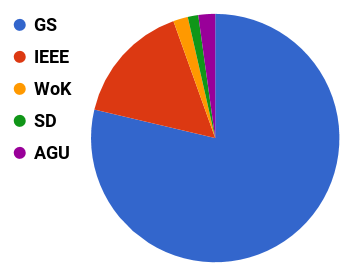
\includegraphics[width=0.4\textwidth]{img/new_results_distribution.png}
    \caption{Results distribution by
    library.}\label{fig:results_distribution}
\end{figure}

Table~\ref{tab:scores} presents the 8 selected articles. It categorises
them with respect to their covered topics and whether they are empirical
or theoretical in nature. The same table summarises article scores
according to the criteria defined in
Subsection~\ref{sub:quality_assessment}, and presents the the keys with
which we will refer to each article from this point forward.

The 8 papers averaged a score of 0,48 and a median score of 0,6. There
is a strong difference between the average and the median suggesting
that there are some outliers or some kind of clustering. Although this
is actually the case, it is statistically irrelevant, given the small
size of the sample.

\begin{table}[htb]
    \centering
    \caption{Scoring results for the selected articles. In the second
    column, a T means the article is theoretical and an E means the
    article is empirical.}
    \label{tab:scores}
    \begin{tabularx}{\textwidth}{lXXXXXr}
        \toprule
        \textbf{Key} & \textbf{Type} & \textbf{Alg.} & \textbf{Inst.} &
        \textbf{Soft.} & \textbf{Cit.} & \textbf{Score}\\
        \midrule
        Hartl2006~\cite{Hartl2006} & T & 1 & 0,4 & 0 & 0,5 & 0,73\\
        Laepple2004~\cite{Laepple2004} & T & 1 & 0 & 0 & 1 & 0,70\\
        Mettendorf2006~\cite{Mettendorf2006} & E & 0,4 & 1 & 1 & 0,25 & 0,57\\
        ODriscoll2003~\cite{ODriscoll2003} & T & 1 & 0 & 0 & 0,25 & 0,63\\
        Olaguer2017~\cite{Olaguer2017} & E & 0 & 0,2 & 0 & 0,25 & 0,07\\
        Poehler (unpub)~\cite{Poehler} & E & 0 & 0,4 & 0 & 0,25 & 0,11\\
        Pundt2005~\cite{Pundt2005} & E & 0,4 & 1 & 1 & 1 & 0,64\\
        Stutz2016~\cite{Stutz2016} & E & 0 & 1 & 1 & 0,25 & 0,33\\ 
        \bottomrule
    \end{tabularx}
\end{table}

% \begin{figure}[htb]
%     \centering
%     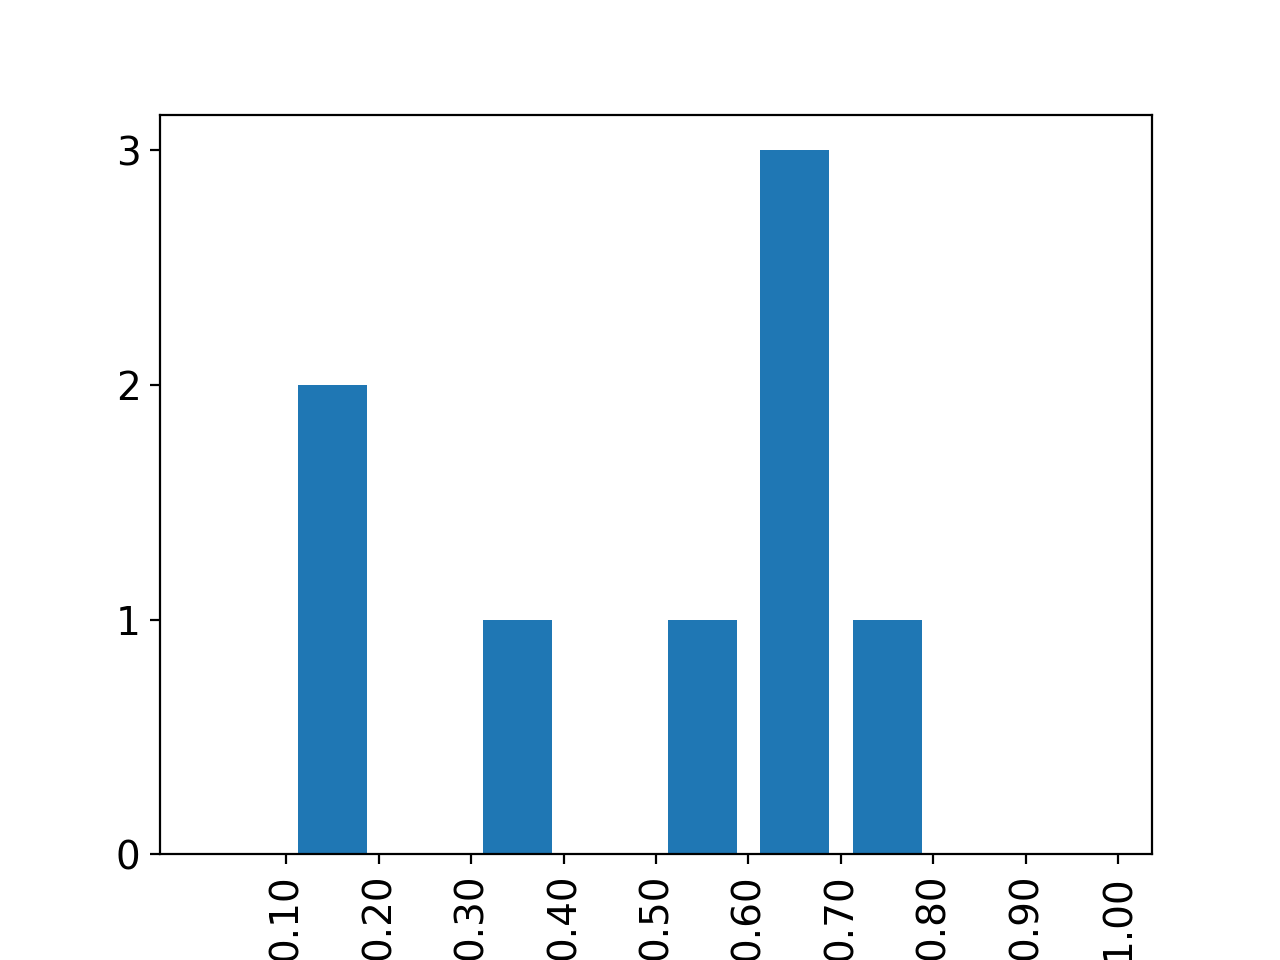
\includegraphics[width=\textwidth]{img/histogram.png}    
%     \caption{Score histogram for the articles in selection.}
%     \label{fig:score_histogram}
% \end{figure}

% \begin{table}[htb]
%     \centering
%     \caption{Article metrics: selection vs whole search.}
%     \label{tab:metrics}
%     \missingtable{Metrics table}
% \end{table}

\subsection{Discussion}
\label{sub:discussion}

In this subsection, we will use the 8 articles that were selected in
order to try and answer the Research Questions. For clarity, we will
approach with respect to the instrument, algorithm and software in a
separate manner.

Different articles present data in different ways, and with different
levels of detail. This has been taken into account in designing our
evaluation method, and it should also be observed when discussing
results. Therefore, our general approach in this subsection will be to
address the more detailed articles first and then complement that
information with what we can gather from the less detailed papers.

\subsubsection{Instrument}
\label{ssub:instrument}

Instrumentation description is present in 7 of the 8
(\cite{Hartl2006,Laepple2004,
Mettendorf2006,Olaguer2017,Poehler,Pundt2005, Stutz2016}) selected
articles. Stutz2016~\cite{Stutz2016}, Pundt2005~\cite{Pundt2005} and
Mettendorf2006~\cite{Mettendorf2006} present the highest level of
detail.

In Stutz2016~\cite{Stutz2016}, the authors used a newly developed Long
Path DOAS instrument for the study of atmospheric concentration of
Benzene, Toluenes and Xylenes. This instrument's main innovation is its
light source, which consists in a double LED (255nm and 265nm) assembly.
This system's telescope is a homebuilt telescope with a focal length of
120 cm and a 12 inch diameter aluminum coated main mirror, mounted on a
high accuracy motorised pan and tilt unit from Newark Systems. The
telescope is used both as emitter and receiver, therefore the system
needs a reflector. Stutz used a quartz corner cube reflector array,
with an individual reflector diameter of 57 mm and the number of
reflector ranging from 10 to 25 (depending on the path length). For
detection, the system relied on a UV-enhanced PIXIS 256 CCD detector
from Princeton Instruments on an Acton spectrometer with 300 grating and
$\approx$0,3 nm spectral resolution, which was stabilised to -35ºC.

Pundt2005~\cite{Pundt2005} was conducted during the BAB II motorway
campaign. The team was working with the goal of performing a tomographic
measurement of vehicle polution along a certain motorway between
Heidelberg and Mannheim. For that, they used an assembly of two
telescopes and eight reflectors, rendering a total of 16 light paths,
then used to perform a tomographic reconstruction of the trace gas
detection in that region. The telescopes used had a focal length of 150
and 80 cm, with respective diameters of 300 and 200 mm. Both assemblies
used Acton spectrometers. One used the Acton 500, with 0,5 nm spectral
resolution in the range between 295 and 375 nm; the other used an Acton
300, with 0,4 nm spectral resolution between 295 and 355 nm. In both
cases, the sensor used was a 1024 pixe Photo Diode Array (PDA),
thermally stabilised at -15ºC. The telescopes were pointed towards two
towers which beared the reflectors, set at heights of 10, 20, 30 and 40
m from the ground. The system's geometry and distances are shown in
Figure~\ref{fig:babii_geometry}.

\begin{figure}[htb]
    \centering
    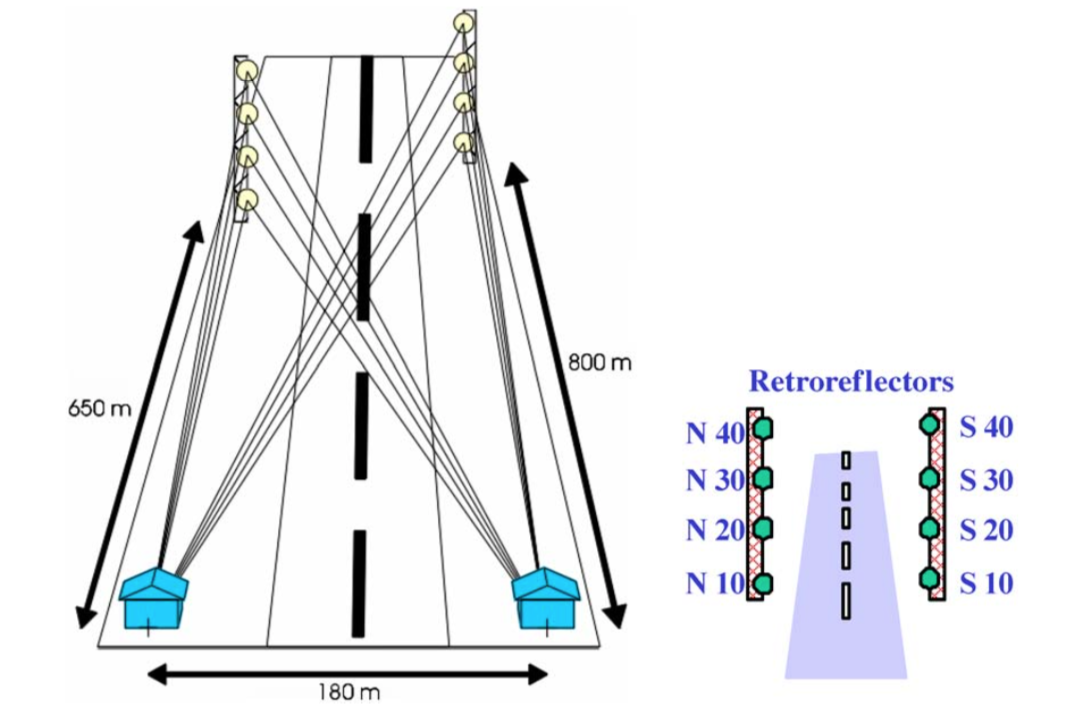
\includegraphics[width=0.8\linewidth]{img/babii_geometry.png}
    \caption{Schematic representation of the BABII campaign
    experiment~\cite{Pundt2005}.}\label{fig:babii_geometry}
\end{figure}

In Mettendorf2006~\cite{Mettendorf2006}, the authors validated
two-dimensional LP-DOAS tomography through an indoor experiment. To this
end, they have used three multibeam instruments, which consisted in a
telescope with a focal length of 1,5 m and 300 mm in diameter, which was
also used as emitter and receiver. The system used a broad spectrum
Xenon lamp as light source, though no details are given. The experiment
assembly included the careful positioning of plane mirrors and 6 cm
diameter corner cube reflectors, used to create a total of 39 light
paths (13 for each multibeam instrument). Telescope, mirror and
reflector positions are illustrated in Figure~\ref{fig:mettendorf_geom}.

\begin{figure}[htb]
    \centering
    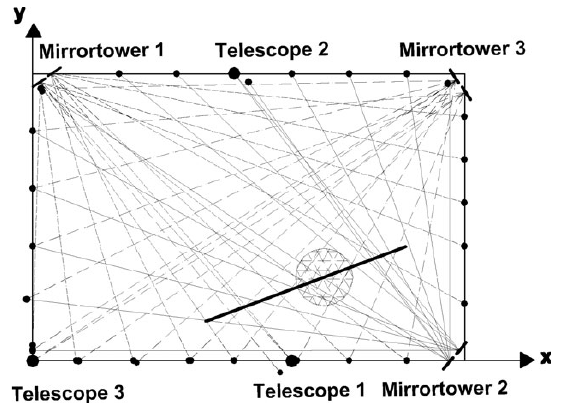
\includegraphics[width=0.8\linewidth]{img/mettendorf.png}
    \caption{Mettendorf2006~\cite{Mettendorf2006} experiment geometry,
    detailing position of telescopes (large filled dots), mirrors (small
lines in upper corners), reflectors (small dots along edges), test
samples (hatched circle), light paths (thin lines) and the movement path
for the sample (thick diagonal line).}\label{fig:mettendorf_geom}
\end{figure}

As for the other 4 less detailed instrument description, three
(Hartl2006~\cite{Hartl2006}, Poehler~\cite{Poehler} and
Laepple2004~\cite{Laepple2004}) are from the same group as
Pundt2005~\cite{Pundt2005} and Mettendorf2006~\cite{Mettendorf2006}, and
therefore use the same or similar hardware.
Olaguer2017~\cite{Olaguer2017}, on the other hand, is the companion
paper of Stutz2016~\cite{Stutz2016}, and therefore gives a description
of the same instrumentation, though in a less detailed manner.

\subsubsection{Algorithm}
\label{ssub:algorithm}

The reconstruction algorithm is the most important part of our study, as
we already demonstrated by the weight it is given in our quality
evaluation model (see Subsection~\ref{sub:quality_assessment}).
Algorithm descriptions are present in 6 of the 8 selected
articles:~\cite{Hartl2006, Laepple2004, Mettendorf2006, ODriscoll2003,
Olaguer2017, Pundt2005}. The most complete descriptions are featured in
Hartl2006~\cite{Hartl2006}, Laepple2004~\cite{Laepple2004} and
ODriscoll2003~\cite{ODriscoll2003}.
Mettendorf2006~\cite{Mettendorf2006}, Olaguer2017~\cite{Olaguer2017} and
Pundt2005~\cite{Pundt2005} approach the reconstruction algorithms with
less emphasis or in a less detailed way.

In Hartl2006~\cite{Hartl2006}, the research team describe their
discretisation process, reconstruction methods, grid translation methods
and error estimation and quality assessment, with the greatest level of
detail being given to the latter.

The paper also focuses in the comparison SIRT and ART results for the
test samples, which consisted in up to four Gaussian concentration
profiles, which were randomly arranged in a 100x100 (a.u.) test field,
in six different geometries and  with up to 36 known light paths.

Furthermore, Hartl2006~\cite{Hartl2006} discusses how the choice of the
reconstruction grid affects both the reconstruction error and
reconstruction area integrals, the possibility of the existence of
background concentration influencing equation constraints and
reconstruction results, and how the whole system would behave were its
geometry any different, namely regarding light paths and number of
telescopes. 

The next algorithm-oriented paper is Laepple2004~\cite{Laepple2004}. In
this article, the group discussed several discretisation approaches,
their drawbacks and advantages. Still on discretisation, they approach
the problem of resolution, and the necessary balance between physical
accuracy and the need for \emph{a priori} information which arises from
increasing it. Afterwards, the group presents some strategies for
solving the linear system that results from discretising the
concentration field and how to take error into account.

For their reconstructions, the group chose to adapt ART, SIRT, and SART
. These adaptations were described and detailed in the article's third
section, before the error estimation procedures adopted in their case.
Finally, the team presents how they chose to optimise reconstruction in
several aspects, including the generation of test plumes and
optimisation for the BABII campaign, which was the parent project of
this article. 

ODriscoll2003~\cite{ODriscoll2003} also covers the algorithm
extensively. While this paper is considerably shorter that the previous
two, it provides a detailed (on an iteration basis) description for ART
and SIRT. In addition, and perhaps of greater interest, the paper's
authors suggest a different approach to solving the reconstruction
matrix, different from the algebric methods already presented: an
evolutionary algorithm.

An evolutionary algorithm is a mathematical method of solving complex
problems, which mimics or is in any form based on the process of natural
selection. These algorithms have, according to the paper's authors and
their references, been shown to be extraordinarily powerful.

The research team have applied a Differential Evolution algorithm to the
reconstruction process and provide a detailed description of how they
have done this.

The other two articles which mention the algorithm are
Mettendorf2006~\cite{Mettendorf2006} and Pundt2005~\cite{Pundt2005}.
Both these studies were conducted under the same project as
Laepple2004~\cite{Laepple2004} and Hartl2006~\cite{Hartl2006} and
therefore their algorithm descriptions and methods draw heavily on
these two studies.


\subsubsection{Software}
\label{ssub:software}

Of the 8 selected articles, only 3 mention the software used. Even these,
do not go into any detail of the reasons that led to that specific
usage. 

In Mettendorf2006~\cite{Mettendorf2006}, the team used TOMOLAB
for the calculation of the modelled column densities of their
experiment. In Pundt2005~\cite{Pundt2005}, spectral analysis was
performed using the \emph{MFC Software}. Finally,
Stutz2016~\cite{Stutz2016} used the DOASIS software for control and
automation purposes, and does not explicitly mention its use for
spectral analysis purposes, although this is likely.

\subsubsection{General Observations}
\label{ssub:general_observations}

While this is not a part of the discussion \emph{per se}, we believe it
makes sense to make some general observations about the data which wwe
had to analyse.

The first important mention is the BABII campaign. This study, which ran
in 2001 and aimed to quantify polution from the A656 motorway between
Heidelberg and Mannheim produced a significant part of the literature
which we analysed.

Another point which should be addressed is that all DOAS tomography
efforts detected in this search were based on active DOAS technology.
This only means that the DOAS systems all employed an artificial light
as a light source.

A final remark is due to the prevalence of algebric methods for
solving the discretisation and reconstruction problem, namely ART, SART
and SIRT. 

\subsection{Validity Threats}
\label{sub:validity_threats}

When writing an MS or an SLR, authors always have to analyse their
findings and methods in order to mitigate potential sources of error or
lack of validity. This is called a validity threat analysis.

There are two main families of validity threats. They can be internal,
i.e., they come from the methods employed used in conducting the study;
or external, which means that the threat comes from the applicability
(or lack thereof) of the effects observed in the study, outside of its
scope.

On the level of internal validity of our study, two main observations
come to mind:
\begin{description}
    
    \item[Relevant papers left out] The very low number of found studies
        could be an indication that our inclusion and exclusion filters
        were set in a too restrictive manner. 
        
        It could also happen that some relevant papers were not found
        due to being written in such a way that the libraries' search
        engines did not find them with our search phrase. This same
        problem would also occur if for some reason, an important
        library was left out of the study, and therefore not searched.

        We mitigate all these risks by selecting a purposefuly broad
        search phrase, by using powerful general search engines (eg.
        Google Scholar) and by running several undocumented test-runs
        with other search phrases.

        A common strategy used for tackling this kind of threat is to
        extend the study through snowballing. In our case, we have opted
        to not perform this operation because of the very high
        cross-reference pattern between studies which we have found.
    
    \item[Quality of selected papers] While it is true that we do not
        have any control over the quality of the articles rendered by
        the search engines, and there is no standard regarding it, we
        must address the issue that it entails. We have tried to
        mitigate this risk, as far as we can, by using strict and strong
        selection criteria in systematic fashion (see
        Section~\ref{sec:methods}).

\end{description}

On the external threat plane, we contend with the applicability of our
findings outside our study. We have tackled this issue by trying to
remaining focused only to the techonologic aspect of the Tomographic
DOAS technique, both in respect to its instrumentation and to the
mathematical methods involved.

With this in mind, and even if the internal validity threats were all
verifiably concerning, this study's finding are of great use to anyone
wanting to understand how the field is working or wishing to design and
build an analysis system.

%!TEX root=../slr.tex
\section{Conclusions}
\label{sec:conclusions}

The initial goal of this study was the assessment of the technological
status of the tomographic DOAS method for atmospheric pollutant mapping,
with the overarching objective of finding an innovative approach to the
subject.  

We have begun by identifying a set of representative electronic
libraries through a preliminary search. Then, we have constructed a
purposefully broad search phrase, which we applied to the selected
libraries. This search has rendered a total of 61 articles, of which
only 13 (around 22\%) were considered relevant and therefore further
studied. The application of the search strategy detailed in
Section~\ref{sec:methods} shows that with the great finding power of
Google's literature-oriented search engine comes an also great need for
scrutiny, since the inherent broadness of the tool results in a large
number of unwanted detections (24 exclusions vs 1 in WoS and 3 in
Scopus).

Our search has found that active tomographic DOAS is far more common
than the passive counterpart (11 out of 13 articles discussed this
method). This preference can be explained by the fact that the results
produced by this kind of system are generally superior to those obtained
by passive methods. However, passive applications are normally much less
demanding on a technical level, and are simpler to run and assemble.
Much as a result of this, we have also identified that the systems used
in the literature were not mobile or had a very low mobility level which
in turn caused that all the systems were working with low projection
numbers (as was identified in several if the selected papers). This
should be taken into account in future research on the topic.

As a final note, we would also like to point out that there seem to be
no commercially available systems for this kind of application, although
some of the articles, like the one by Stutz in 2016~\cite{Stutz2016}
detail systems which could easily be adapted to that end.







